\documentclass[12pt]{report}
\usepackage{common}
\usepackage[round]{natbib}
\usepackage[strings]{underscore}
\usepackage{url}
\usepackage{todonotes}
\usepackage[toc]{appendix}
\usepackage{setspace}
\usepackage{hyperref}
\usepackage[english]{babel}
\usepackage{amsthm}
\usepackage{caption}

\newcommand\numberthis{\addtocounter{equation}{1}\tag{\theequation}}
\newtheorem{theorem}{Theorem}




%\title{Coarse-to-Fine Attention Models for Document Summarization}
%\author{Jeffrey Ling}
%\date{}
\begin{document}
\pagenumbering{roman}


\begin{titlepage}
	\centering
	\vspace*{2cm}
	{\Huge\bfseries Coarse-to-Fine Attention Models for \\
				Document Summarization \par}
%	\includegraphics[width=0.15\textwidth]{example-image-1x1}\par\vspace{1cm}	\vspace{1cm}
	\vfill
	{\LARGE Jeffrey Ling\par}
	\vspace{1cm}
	{\Large A Senior Thesis for the \\
		Joint Concentration in \\
	Computer Science \& Mathematics\par}
	\vspace{1cm}
	{\Large Harvard College\par}
	\vspace{1cm}
	{\Large \today }

	\vfill

% Bottom of the page
%	{\large \today\par}
\end{titlepage}
%\maketitle{}
\onehalfspacing

% dedication
\clearpage
\thispagestyle{empty}
\vspace*{4cm}
\begin{center}
 Dedicated to Leland and Brandon
\end{center}
\clearpage


% acknowledgements
\clearpage
\thispagestyle{empty}
\vspace*{2cm}
\begin{center}
\LARGE\bf Acknowledgements
\end{center}
\vspace{1cm}

To Prof. Sasha Rush for his invaluable advising for the past two years. None of this work would be possible without his encouragement and mentorship.

To the graduate students of our lab for a fun and friendly research experience, especially Yoon Kim for his life advice, encyclopedic knowledge of tuning deep neural networks, and constant availability on Slack,
and Yuntian Deng for his unyielding optimism that kept my experiments going.

To my thesis readers, Profs. David Parkes and Stuart Shieber, for agreeing to review this incredibly long piece of writing.

To the math library and my cohorts there. Silence is golden.

To my peers for supporting a lively learning environment, especially Rachit for always having a moment for an interesting discussion.

To my roommates, Kenneth and Andres, for not judging me when I returned from the distant land of the quad.

To my parents, who gave their hearts and souls to get me where I am today, and my brothers, who have grown a little bit too tall since I was last home.

To Sindy, for standing by me in just about every way possible.


\clearpage % For letting the acknowledgements appear on a separate page


\begin{abstract} % needs work
While humans are naturally able to produce high-level summaries upon reading paragraphs of text, computers still find such a task enormously difficult. Despite progress over the years, the general problem of document summarization remains mostly unsolved, and even simple models prove to be hard to beat.

Inspired by recent work in deep learning, we apply the sequence-to-sequence model with attention to the summarization problem. While sequence-to-sequence models are successful in a variety of natural language processing tasks, the computation does not scale well to problems with long sequences such as documents. To address this, we propose a novel coarse-to-fine attention model to reduce the computational complexity of the standard attention model.
%By organizing the source sequence into a 2-dimensional image, we hierarchically apply attention, using a coarse mechanism for the first layer to select a row sequence, and a finer mechanism for the second soft attention layer. While the computation for training standard seq2seq models scales linearly with source sequence length, our method is invariant to length and thus can scale arbitrarily.

We experiment with our model on the CNN/Dailymail document summarization dataset. We find that while coarse-to-fine attention models lag behind state-of-the-art baselines, our method learns the desired behavior of attending to subsets of the document for generation.
Therefore, we are optimistic that the general approach is viable as an approximation to state-of-the-art models. We believe that our method can be applied to a broad variety of NLP tasks to reduce the cost of training expensive deep models.
\end{abstract}

\tableofcontents{}

\listoffigures

\listoftables




\chapter{Introduction}

\pagenumbering{arabic}

\section{Natural Language Processing}

The field of natural language processing arises from a very simple question: how can we teach machines to read, speak, and understand the words that we use with such ease and fluency?

Such a question has been considered since the first computers were built. The classic Turing test, posed by Alan Turing in 1950, requires a machine to converse in a way that is indistinguishable from a human, and thus requires a fundamental grasp on how to properly use language.
Although it was simple for Turing to conceptualize what a successful machine might look like, many have been stumped on how to actually construct such a system.
Indeed, to this day, no machine has been able to fully pass the Turing test as it was originally posed.


While computers can now run computations at a rate that far exceeds human cognition, language tasks that we consider trivial still prove to be extraordinarily difficult for a machine to solve. Consider the problem of deciding words with multiple meanings such as ``bass'' (word sense disambiguation), or the problem of identifying to what or whom a certain pronoun refers (coreference). 
While humans reliably perform these functions on a daily basis, they are not at all easy for computers to handle.


However, the need for computers to understand language has never been greater.
In today's information age, NLP grows increasingly important as the accumulation of free-form text begins to outpace the ability of humans to process it. In fields such as medicine, this can mean missed diagnoses; in law, wasted effort on irrelevant documents; in international relations, misinterpretations of foreign articles.
Because natural language is everywhere and used by everyone, the demand for text processing solutions remains as high as ever.

\section{Methods in NLP}

In this section, we investigate the general philosophy of tackling NLP problems.

The key property of language that makes it difficult for machines to handle is its discrete and combinatorial nature. When we form sentences, we can string together arbitrary words from our vocabulary, as long as we follow the rules of some highly structured grammar. In some sense, the essential difficulty in NLP lies in handling these complicated structures in an efficient way.

Linguistics attempts to provide an answer by building a formal theory of language. Indeed, many ideas from linguistics, including sentence parses, morphology, and semantics are invaluable in NLP for understanding how sentences and phrases are put together.
In order to solve a language problem, we might begin by enriching the surface form of text (the raw sentences and paragraphs) with the parse structure, parts of speech, coreferent entities, etc. We can then use this featurized form of language in whichever way we prefer.

\begin{figure}[t]
\centering
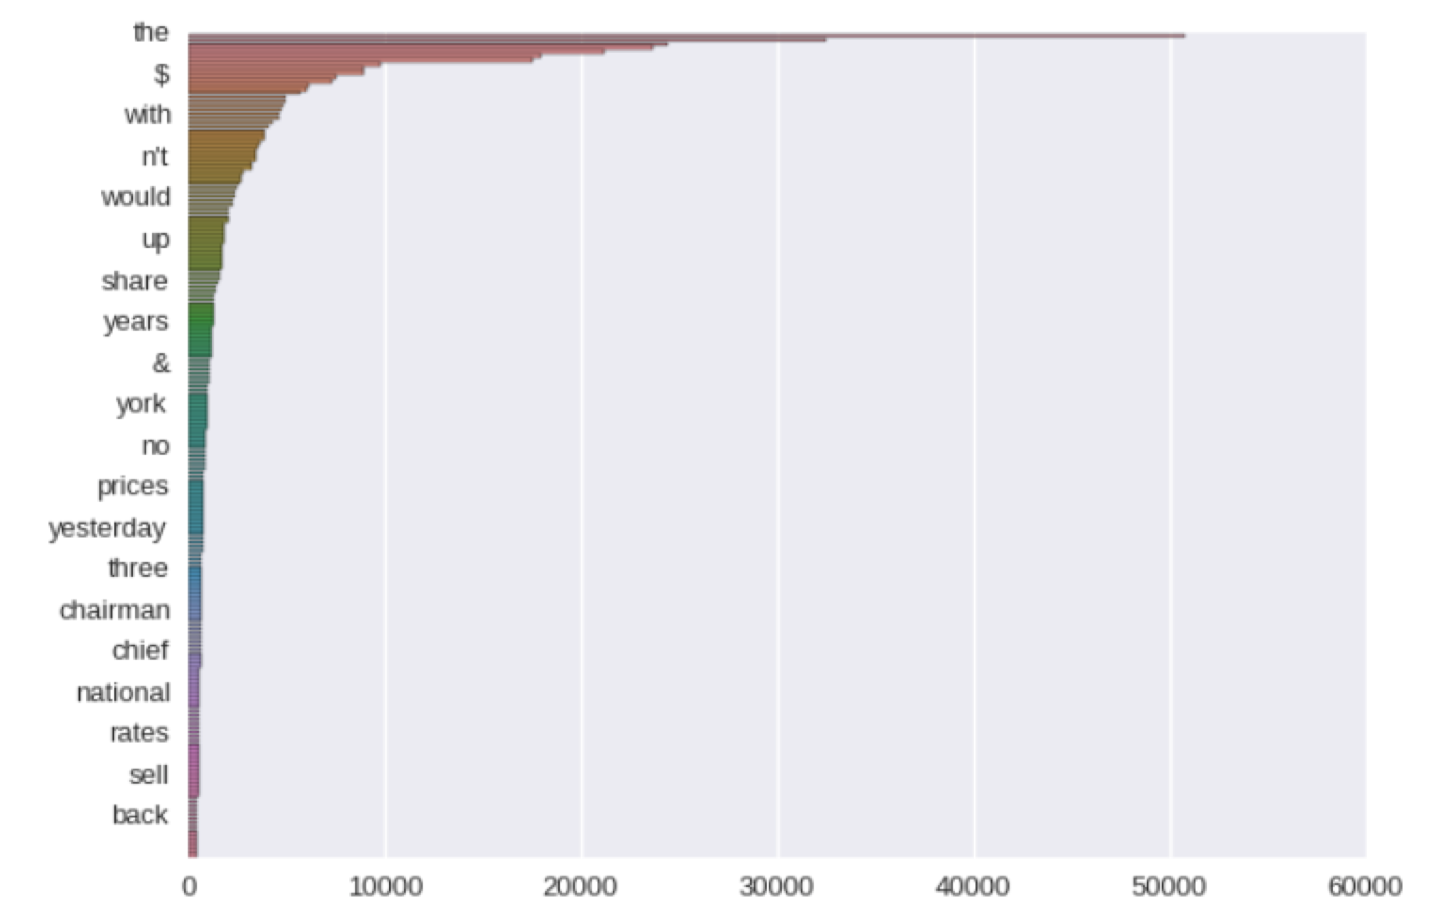
\includegraphics[scale=0.5]{images/zipf}
\caption[Zipf's Law]{Zipf's law, indicating the relationship between English words and their frequency. The distribution approximately follows an inverse power law. Image from CS287.}
\label{fig:zipf}
\end{figure}

Another mode of thought focuses on the role of statistics in language. A cursory examination of the distribution of English words reveals an interesting power law distribution known as Zipf's law (Figure~\ref{fig:zipf}). By drawing from ideas of information theory \citep{Shannon1948}, we can treat language as the result of some noisy probabilistic process, and we can reduce problems such as language modeling to learning the parameters of some simple distributions.

Historically, there has been contention about the roles of linguistics and statistics in NLP. Certain practical problems seem to be better off without linguistic theory; as IBM researcher Frederick Jelinek famously said, ``Every time I fire a linguist, the performance of the speech recognizer goes up'' \citep{Jurafsky2009}. Indeed, even naive models of language perform well if given enough training data, as evidenced by the IBM models for machine translation \citep{Brown1993}.

Today, the linguistics-free approach has been taken to an extreme by deep learning systems. For the first time, neural networks are able to learn to perform language tasks in an end-to-end fashion \citep{Collobert2011}, i.e. without the linguistic preprocessing that was once considered necessary.
Neural methods have been adopted by user-facing systems like Google Translate with great success \citep{GoogleTranslate2016}.


\section{Automatic Summarization}
\label{sec:taxonomy}

In this thesis, we will consider the particular problem of \emph{text summarization}.
That is, given a document with several sentences of text, the goal is to produce a concise and fluent summary that captures most of its salient points.

Text summarization is one of the biggest open problems in NLP, as identifying the key information of a document seems to require a deep understanding of its content. Nevertheless, there is an urgent need for successful summarization algorithms in the text-dominated discourse of the modern era.

\citet{Nenkova2011} give a comprehensive overview of the problem of summarization. In particular, they provide a taxonomy of methods that researchers have developed to tackle the task:

\paragraph{Extractive vs. abstractive} Extractive summaries extract certain sentences or phrases from the document with minimal further processing, while abstractive summaries might include paraphrasing and original word choice (similar to how humans produce summaries). 

Extractive methods are by far more popular due to the simplicity of building an extraction algorithm. Abstractive methods are much more difficult, as we need to both capture the critical pieces of information and also ensure grammaticality of the output (a difficult problem in itself).

\paragraph{Single- vs. multi-document} Summarization was originally posed as the problem of producing a summary for a single document. However, with the onset of the Internet, there are often multiple documents on the same topic, and so a summarization system should be able to combine them to produce a summary.

Interestingly, \citet{Nenkova2011} note that the multi-document problem is often easier due to redundant information across sources. In contrast, in the single-document problem, a crucial piece of knowledge might only be repeated once.

%\paragraph{Indicative (style) vs. informative (facts)} Indicative summaries provide a sense for what a certain document is about without necessarily giving all of its details, while informative summaries are meant to replace the original document in terms of content.

%\paragraph{Keyword vs. headline} Keyword summaries are allowed to simply be a bag-of-words of important keywords from the document, while headline summaries must form a coherent sentence.

\paragraph{Generic vs. query-focused} Generic summaries make no assumptions about the reader and are meant to be generally informative, while query-focused summaries take into consideration a query and only return relevant information from the document.

The contrast between these two methods highlights an important question in summarization: to what end are we summarizing documents? If we can answer this question, we can build systems to more accurately accomplish our desired tasks.

\vspace{0.5cm}


Most of this taxonomy is based upon insights from DUC (Document Understanding Conferences), a set of tasks released by NIST between 2001-2006 to promote research in summarization \citep{over2007duc}.

The DUC tasks were fairly diverse and varied from year to year. DUC 2001 and 2002 asked for generic summaries of news articles, while DUC 2003 presented a multi-document problem. DUC 2004-2006 shifted to a more question-answering based approach, and many of the documents were accompanied by focused queries.

While DUC did not lead to any definitive answers on how best to summarize documents, some important empirical discoveries were noted.
For the generic summarization tasks, it was observed that the first sentence of news articles was a strong baseline that more sophisticated methods found hard to beat. Thus, the generic summary task was seen as ill-formed and not as interesting, leading to the more query-focused tasks in the later years.


DUC also inspired a lot of thinking on how to best evaluate summaries. Evaluating a summary is inherently ambiguous, as even humans tend to disagree on what makes for a good summary.
While a single best quantitative metric may not exist, DUC established several important criteria, including grammaticality, non-redundancy, and content coverage.

One proposed metric for evaluation is recall on elementary discourse units (EDUs), labeled clauses within a summary that ought to be captured. Unfortunately, this method requires the data to be labeled with clauses. ROUGE \citep{lin2004rouge}, inspired by the BLEU metric for machine translation \citep{Papineni2002}, is a cheap and fast method based on overlapping n-grams, and does not require any additional annotation. Due to its ease of use, ROUGE is one of the most popular evaluation metrics today.

%For extractive summaries, people have proposed simple metrics such as precision and recall on selected sentences. These naturally do not work too well since 1) not all sentences are equally informative, and 2) not all parts of a sentence are relevant.
%When we don't have sentence labels as in the extractive case, evaluation is harder.



While useful, none of these metrics directly address the grammaticality of the output. Aside from using human evaluation, meaningful metrics for summaries is still very much an open question \citep{toutanova2016summarymetrics}.


\vspace{0.5cm}

 

%It is important to highlight these differences to understand how people thought about the problem. The complexity of this taxonomy indicates that the summarization problem in its simplest formulation is very poorly defined. Indeed, query-focused summarization may well be a useful task, but it may be more accurate to classify it as question-answering rather than summarization.


Going forward, we will limit our scope to the single-document and generic summarization case. We will explore some related work in extractive and abstractive summarization, then connect these approaches with recent trends in deep learning.

\section{Related Work}

One of the first treatises on automatically producing summaries was \citet{luhn1958automatic}, which considered the problem of producing abstracts for scientific articles. At the time, computers were still monolithic machines that ran on punch cards, so automating the summarization process was quite ahead of its time.

\citet{luhn1958automatic} proposed a simple sentence-ranking method to produce summaries. The algorithm gives each sentence a score based on the occurrence of frequently appearing words. This is one of the first examples of an extractive summarization method.

Since then, a variety of approaches have been applied. We highlight some notable work in both the extractive and abstractive frameworks.

\subsection{Extractive}
The most popular methods for document summarization have generally been extractive due to their simplicity.

There are two natural procedures for extractive summarization: one is to produce a ranking of sentences based on some scoring function, and the other is to train a binary classifier on whether a sentence should be in the summary. \citet{luhn1958automatic} is an example of the first approach.

\citet{Carbonell1998} extend on the scoring-ranking method with an information metric, MMR (maximum marginal relevance), that penalizes pairwise similarity between sentences. Their work is one of the first that attempt to reduce redundancy in the summary.

\citet{Kupiec1995} pioneer the second method by treating sentence selection as a classification problem, training a naive Bayes classifier on sentences.

Ranking and classifying algorithms have generally become more sophisticated over time. Today, deep learning systems prove to be some of the most powerful classifiers, and some have found applications in extractive summarization.
\citet{Cao2015} use convolutional neural networks to extract features for each sentence, combining these with document-level features to produce ranking scores.
\citet{Cheng2016} apply the encoder-decoder model using recurrent neural networks to jointly produce labels for each sentence.

One key drawback of these trained extractive models, especially the deep ones, is the scarcity of annotated data. In extractive models, we require sentences of each document to be labeled as positive or negative in order to train a classifier, and data in this format can be hard to obtain.

%\citet{Shen2004} models sentence extraction as a sequential classification problem, training a linear-chain conditional random field to find the best subset of sentences.
%
% 
%\citet{svore2007} use a basic neural network as a sentence classifier.




\subsection{Abstractive} While extraction has proven to be successful, the method is inherently limited in its ability to summarize. The more challenging method, and also the closest to what humans do, is \emph{abstractive} summarization. Instead of strictly requiring the summary to be a subset of the source document, any coherent text is allowed.

Because generative models of language were historically not very powerful, the main techniques used to produce abstractive summaries involved extraction followed by sentence compression.
 \citet{knight2002summarization} employ a noisy channel model and probabilistic context-free grammars to deduce the ``most probable'' compression of a sentence.
%while \citet{clarke2008global} uses an integer linear program.
\citet{cohn2008sentence} extend the grammar-based method to allow for insertions and substitutions during compression, whereas prior methods were purely deletion based.
\citet{zajic2004topiary} combine sentence compression with an unsupervised topic detection algorithm to achieve the best result on DUC 2004.
Recently, \citet{Durrett2016} apply an integer linear programming (ILP) approach, where they extract phrases according to a feature-based scoring function and merge them with grammaticality constraints.

%Fusion: align parse trees and combine phrases that are similar

We note that because these methods rely heavily on a strong extraction system, they might not qualify as truly ``abstractive.'' Deep learning models, however, have been very successful at building generative models of language, and have naturally found applications in abstractive summarization. \citet{rush2015neural} propose a completely data-driven model for headline generation by training an end-to-end model. More recently, \citet{nallapati2016seq2seq} apply the same approach on full documents.

As with deep learning methods for extraction, these models require a large amount of supervised training data. One advantage of the abstractive model is that data in the document-abstract format is more easily obtainable than labeled extractive data.


\subsection{In the Wild}

Outside of the academic realm, summarization is an important problem in industry. One noteworthy summarization method is on Reddit\footnote{reddit.com}: in order to summarize long forum discussions, Reddit uses technology from Smmry\footnote{smmry.com}.

Smmry's algorithm is a simple extractive method. It counts word occurrences, splits discussions by sentence, and ranks the sentences based on the sum of their word scores. This algorithm bears extraordinary similarity to \citet{luhn1958automatic} --- although a variety of work has been done since then, the simplest approaches turn out to be the most practical.

\section{This Work}

Inspired by advances in deep learning for NLP and dissatisfied by the limitations of extractive models, we set out to build a deep model to abstractively generate summaries for documents. Because deep learning is computationally expensive even for short lengths of text, this creates a challenge for the general document summarization problem.

Hence, we will survey the literature for methods that alleviate the computation of training deep models. Along the way, we propose a new model architecture that extends the popular sequence-to-sequence attention model in NLP and attempts to reduce the computational complexity of the document summarization problem.

\section{Outline}


We provide an outline for the rest of this thesis.

In Chapter~\ref{chap:background}, we give a survey of deep learning and motivate its use in solving our problem. We also provide the necessary background material for understanding our models and algorithms.
In Chapter~\ref{chap:algorithms}, we describe our training algorithm formally.
In Chapter~\ref{chap:models}, we describe our models formally.
In Chapter~\ref{chap:experiments}, we describe the experimental setup, including our dataset and baselines. %, and practical details for training our models.
In Chapter~\ref{chap:results}, we show results and analyze the outputs of our models.
In Chapter~\ref{chap:discussion}, we discuss our results.
Finally, we conclude in Chapter~\ref{chap:conclusion}.

%%%%%%%%%%

\chapter{Background}
\label{chap:background}

In this chapter, we give a brief primer on deep learning and representation learning in the context of NLP.

Then, we set up the relevant background ideas for our models. We describe the popular sequence-to-sequence attention model at a high level, then survey the literature for methods in reducing the computational cost of deep models. Finally, we introduce the framework of reinforcement learning, which will provide the foundation for one of these methods.


\section{Deep Learning}

The history of neural networks dates back to the perceptron \citep{Rosenblatt1958}, a simple model that assumes data can be linearly separated. Due to this strict requirement, the machine learning community dismissed the idea as impractical for most of the 20th century.

%Later, \citet{Rumelhart1986} showed that the backpropagation algorithm could be used to efficiently train general neural networks, reviving interest in the subject. However, this was before the era of GPUs and modern computing, and so the algorithm could not be put to practical use.

Recently, neural networks have made a resurgence. In the ImageNet image classification competition in 2012, \citet{Krizhevsky2012} won using deep convolutional neural networks \citep{LeCun1995}, beating the competition by a significant margin. This led to a renewed wave of research, especially due to the advancement of GPU computing power, which can train networks at 10 to 20 times the speed of standard CPUs. Today, deep models are successfully used in image recognition \citep{Farabet2013}, speech recognition \citep{Hinton2012}, and Go playing \citep{Silver2016}, just to name a few.


In NLP,  \citet{Bengio2003} first demonstrated the viability of deep models by building a neural language model using multi-layered perceptrons. Later, \citet{Collobert2011} show that neural models can be used to train end-to-end models without any of the preprocessing that was once considered necessary.

Since their onset, deep models have found their way into nearly every corner of NLP. Much of their success relies on the ubiquity of the \emph{long short-term memory} (LSTM) recurrent neural network \citep{hochreiter1997long}, a model used to both process and generate sequences of text, and \emph{word vectors}, distributed vector representations of text.
Several state-of-the-art algorithms are now based upon these deep learning tools; while there is too much to cover here, \citet{goldberg2015primer} provides a concise summary of the models that have had the greatest impact on NLP. % weak

\section{Representation Learning}

While neural networks are often treated as black box classifiers, \citet{Zeiler2014} show that the intermediate layers of deep convolutional networks in computer vision contain abstracted qualities of the input, such as patterns, textures, and objects. This suggests that neural networks are discovering latent features and building generalized \emph{representations} of their inputs.

\begin{figure}[p]
\centering
\includegraphics[trim={20cm 20cm 20cm 20cm},clip,width=\textwidth]{images/graph}
\caption[Word2vec Clusters]{A visualization of word2vec word vectors \citep{mikolov2013word2vec}, projected to two dimensional space using PCA. Words with similar semantic meaning tend to cluster together in the space. Image from CS287.}
\label{fig:word2vec}
\end{figure}

The idea of learning representations of the input also applies in NLP.
\citet{mikolov2013word2vec} show that by training an unsupervised neural network on a Google News text corpus, the network learns to map words in the English language to vectors of real numbers known as \emph{word embeddings}.
These word embeddings are actually able to capture semantic properties of the words --- for example, taking the vectors for \emph{king}, \emph{man}, and \emph{woman}, we find that $v_{king} - v_{man} + v_{woman} \approx v_{queen}$, preserving the analogy that we usually make in English. Figure~\ref{fig:word2vec} shows some of the word2vec vectors when projected to two dimensional space.

Representation learning has since become a central topic in NLP. Word vectors trained on a general text corpus can be used in almost any NLP model \citep{mikolov2013word2vec, Pennington2014}, and the task-invariant property of these vectors is highly attractive.
It remains to be seen whether it's possible to represent longer pieces of text, such as sentences, in a general way, and research in the area is active \citep{Bowman2016}.

%\section{Summary}
%
%We consider some recent work done in deep neural summarization.
%
%We can frame summarization as a supervised headline generation problem. That is, given a document (the source sequence of words), we desire to produce a shorter headline or summary (the target sequence). 
%
%
%Existing methods in deep learning have proven to be highly effective for this kind of task, especially the sequence-to-sequence (seq2seq) model \citep{sutskever2014sequence, bahdanau2014neural}. 
%
%\citet{rush2015neural} use the seq2seq model to summarize single sentences into headlines, but we consider the more general problem of summarizing arbitrarily long documents.
%
%More recently, seq2seq models have been applied to train both extractive \citep{} and abstractive \citet{nallapati2016seq2seq} summarization systems at the document level. While such work demonstrates the feasibility of deep learning in this problem, it is very preliminary and leaves much room to explore alternative architectures.




\section{Motivation}


Why deep models? There are currently two general approaches to solving problems in NLP: one is to use as much linguistic theory as possible to reduce the problem, and another is to apply black box learners such as deep neural networks.

Deep models work fantastically well on many tasks, especially when it comes to improving on metrics, and one might wonder if there is even a need to consider other models. However, as big of a hammer as deep learning is, it is useless without nails to hit.
That is, in order to further language understanding, datasets and tasks must be posed such that deep models can be applied; it is exactly in this domain that classical theory is still relevant.
As \citet{Manning2016} argues, although neural models have come to dominate NLP papers, there will always be a need for domain experts to prepare the field so that deep learning can succeed.

%On one hand, systems with handcrafted features can perform extremely well if domain specific knowledge can be built in.
%On the other hand, a purely data-driven system can automatically create most of the necessary features, and empirically are proven to work very well.

With this caveat, there are many worthwhile reasons to study deep networks in NLP. First, they work! In fact, they work remarkably well without any feature engineering, which tends to be one of the fussiest parts of building machine learning algorithms.

Second, they are not mutually exclusive with standard feature extraction methods, and so can augment classical methods.

Third, we find that trained models can discover latent structure in language automatically, which may reveal insights about how language is used. For example, word vectors tend to cluster around semantic concepts without any direct supervision.
%As an example, sequence-to-sequence models with attention \citep{bahdanau2014neural} learn the concept of a word alignment in translation without any direct supervision.


It is this third point upon which we base this thesis. Although they began as black-box optimizers, end-to-end deep models are slowly being dissected into more understandable parts. One of our goals is to test the hypothesis that such parts are in fact interpretable and are functioning as we expect them to.

With this goal in mind, we attempt to interpretably extend the attention mechanism of the popular \emph{sequence-to-sequence models}. In the next section, we describe the sequence-to-sequence model informally to gain intuition on how it works.


%\todo{needs work} 



\section{Sequence-to-Sequence Attention Models}

Many NLP problems can be posed as follows: given an input sequence of tokens $\boldx = x_1, \ldots, x_n$ with $x_i \in \mcX$, we train a model to produce an output sequence $\boldy = y_1, \ldots, y_m$ with $y_j \in \mcY$. We normally pose this as a probabilistic problem and model the conditional probabilities, so that we wish to find
\begin{equation}
\begin{split}
&\argmax_{\boldy \in \mcY^m} p(y_1, \ldots, y_m | x_1, \ldots, x_n) \\
= & \argmax_{y_1, \ldots, y_m \in \mcY} p(y_1 | \boldx)p(y_2 | y_1, \boldx) \cdots p(y_m | y_1, \ldots, y_{m-1}, \boldx)
\end{split}
\end{equation}

The sequence-to-sequence architecture of \citet{sutskever2014sequence}, also known as the encoder-decoder architecture or seq2seq, neatly provides a solution to this framework. By encoding the input $x_1, \ldots, x_n$ into a fixed size vector which we call the \emph{context vector}, we can compute the conditional probabilities and hence generate $y_1, \ldots, y_m$.
This model has been used to great effect in a variety of NLP tasks, including machine translation \citep{sutskever2014sequence, bahdanau2014neural}, question answering \citep{Hermann2015}, dialogue \citep{li2016persona}, caption generation \citep{xu2015captioning}, and in particular summarization \citep{rush2015neural}.


A popular variant of sequence-to-sequence models are \emph{attention} models \citep{bahdanau2014neural}. Instead of mashing the input into a single context vector, we instead keep an encoded representation of each part of the input, ``attending'' to the relevant part each time we produce an output from the decoder. In practice, this means computing attention weights for all encoder hidden states, then taking the weighted average as our new context vector.
%If we have a representation $\boldh_i \in \reals^d$ for input token $x_i$, we model this attention process by computing weights $\alpha_1, \ldots, \alpha_n$ such that $\sum_{i=1}^n \alpha_i = 1$. The resulting context vector is then the weighted average $\sum_{i=1}^n \alpha_i \boldh_i$.

\begin{figure}[t]
\centering
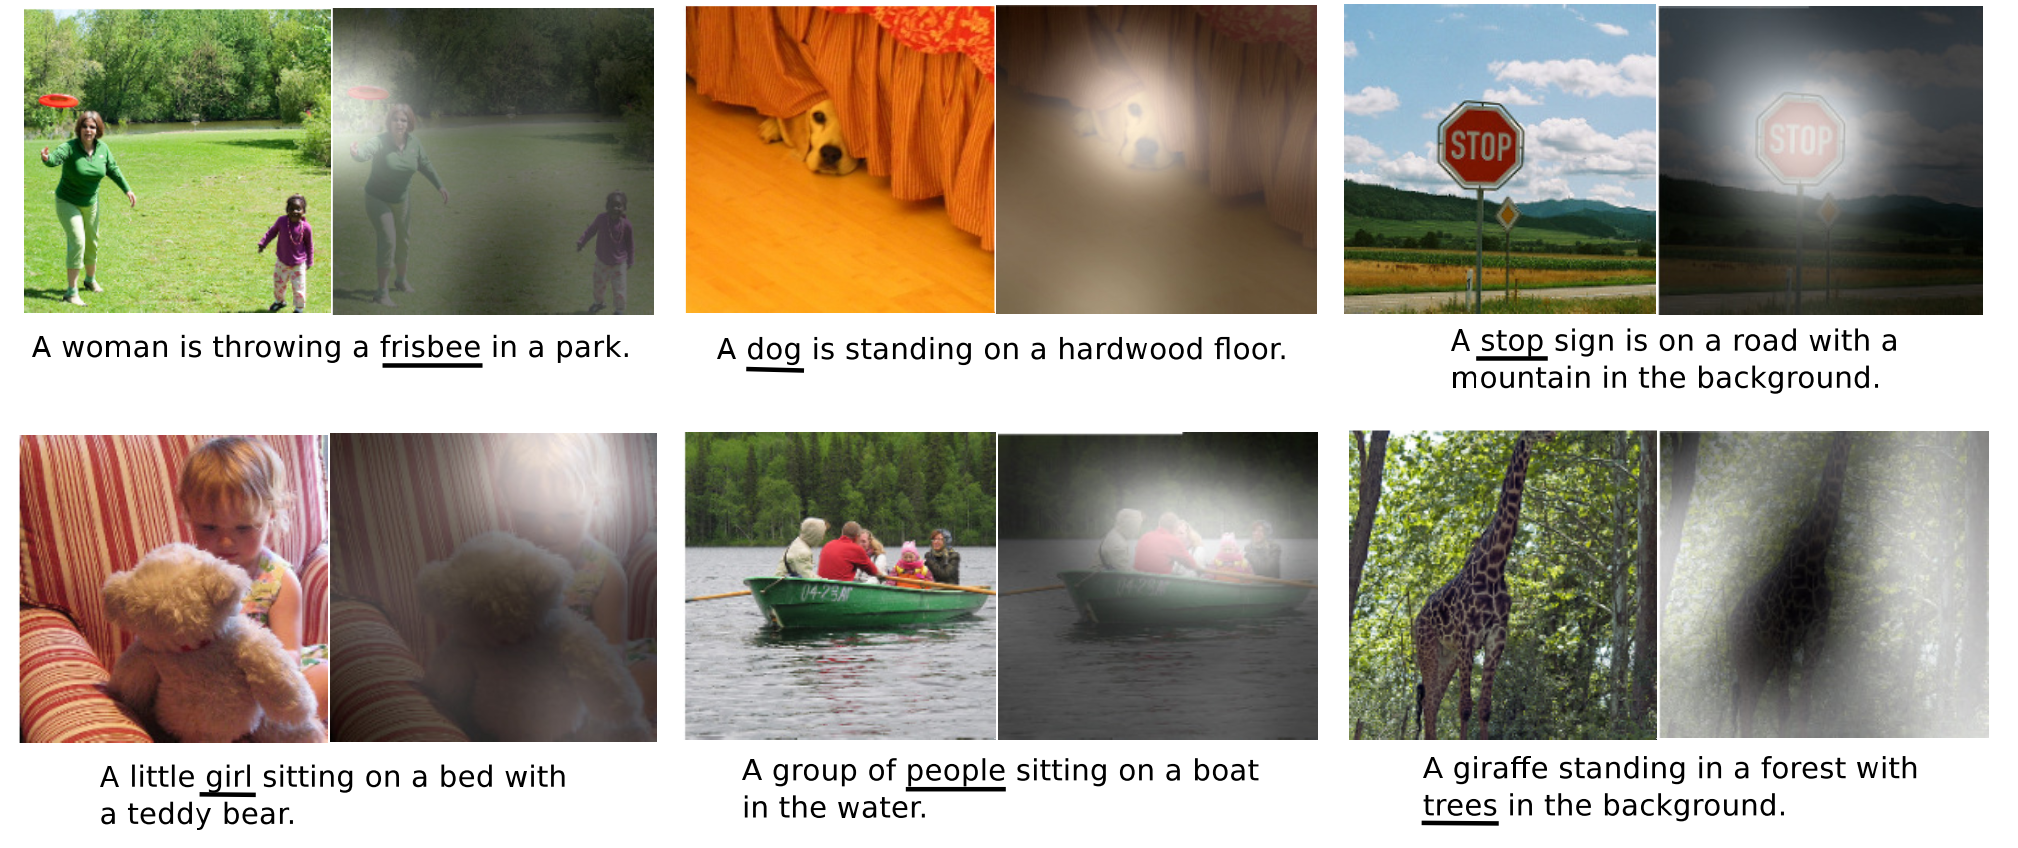
\includegraphics[width=\textwidth]{images/xucaption}
\caption[Attention for Image Captioning]{Attention of a caption generating neural model \citep{xu2015captioning}. The model learns to highlight the correct object when generating words.}
\label{fig:caption}
\end{figure}

\citet{xu2015captioning} show how attention models can be used to ``summarize'' an image and produce a caption (Figure ~\ref{fig:caption}). 
By analyzing where in the image their models attend to when generating each word of the caption, i.e. where the attention weights are highest in the image, they qualitatively find that the model is essentially describing certain objects.



While successful, existing seq2seq methods are limited by the length of source and target sequences. For a problem such as document summarization, the source sequence of length $N$ requires $O(N)$ model computations to encode, where $N$ could potentially be very large. However, it makes sense intuitively that not every word of the source will be necessary for generating a summary, and so we would like to reduce the amount of necessary computations over the source.

Therefore, in order to scale seq2seq methods for this problem, we aim to prune down the length of the source sequence in an intelligent way. The natural solution is to force the model to only use a subset of the input rather than naively encoding the entire input. We investigate some related work in this area.


\section{Conditional Computation}


%The problem of full document summarization, however, is still very open. In order to make the models work, \cite{nallapati2016seq2seq} use a variety of tricks: limiting the decoder vocabulary to the document, the use of pointer attention for \texttt{<unk>} tokens, etc. Our goal in this paper is not necessarily to optimize performance, but to understand how to scale up existing seq2seq methods in an efficient way, and so we attempt to eliminate the use of these ad-hoc tricks whenever possible. We aim to find the best implementation of ``hard'' attention, in which a discrete subset of the source document is selected at any given time, to satisfy the scalability condition.


Many techniques have been proposed in the literature to efficiently handle the problem of large inputs to deep neural networks, and we consider the particular framework of conditional computation.

The term ``conditional computation'' was coined by \citet{BengioLC13} --- the idea is to only compute a subset of a network for a given input. 
To this end, \citet{BengioLC13} propose the use of stochastic nodes in the network to implement discrete random variables, which serve as gates to turn on or off certain parts of the network for computation.
Unfortunately, discrete variables cannot be backpropagated through as they produce zero gradient, and so \citet{BengioLC13} suggest the naive \emph{straight-through} estimator for binary stochastic gates.
In the forward step of the network, they simply sample from the stochastic gates, and backpropagate the gradient as if they had not sampled.

Many alternative methods, some deterministic and some stochastic, have been proposed for conditional computation. 

On the stochastic front, we usually want to sample from a multinomial distribution, i.e. select one choice out of multiple choices, to conditionally compute. In deep networks, the softmax function $\operatorname{softmax} : \reals^m \to [0,1]^m$ is used to produce a normalized probability distribution out of any vector of reals. For $\boldz \in \reals^m$,
\begin{equation}
\operatorname{softmax}(\boldz)_i = \frac{\exp(z_i)}{\sum_j \exp(z_j)}
\end{equation}
We can sample from this distribution to decide which parts of the network to compute. To train the model, we will require methods from reinforcement learning, which we cover in the next section. \citet{xu2015captioning} apply this technique in the form of ``hard'' attention --- while standard ``soft'' attention averages the representations of where the model attends to, in hard attention we discretely select a single location.
This approach has also been applied by others for computer vision tasks \citep{mnih2014visualattention, ba2015visualattention}.

%As an alternative to reinforcement learning, \citet{Maddison2017} apply a smoothed version of the Gumbel max trick in order to approximate the sampling process. The Gumbel max trick is an alternative method for sampling multinomial random variables: by drawing i.i.d. uniform variables $U_i \sim \mathrm{Unif}(0,1)$, taking the argmax of $z_i - \log(-\log(U_i))$ gives us a sample with the correct probability. While this process is still discrete and has no gradient, \citet{Maddison2017} use a softmax instead of a max to obtain a smooth approximation that can be differentiated.


On the deterministic front, \citet{rae2016sparsememory} use an approximate nearest neighbors approach for their ``sparse access memory'' model to train a large-scale neural Turing machine.
\citet{Shazeer2017} introduce a mixture-of-experts model that deterministically chooses a subset of ``expert'' networks to train at any given time.
The key-value memory networks of \citet{Miller2016} select subsets of text by computing word overlap; this process, however, is not learned.
 \citet{martins2016sparsemax} propose the \emph{sparsemax} function as a substitute for softmax, which projects a given vector of weights to the probability simplex. It turns out that this function is differentiable and also has sparse output; however, we are not guaranteed to have a one-hot vector as we get from sampling the multinomial distribution.


\section{Reinforcement Learning}

Standard backpropagation training of neural networks assumes that the output is a deterministic and differentiable function of the input. Reinforcement learning, however, is a more general framework that makes no such assumptions.

The traditional setup of reinforcement learning (RL) assumes some agent is navigating an environment and earning rewards.
We assume a state space $\mcS$, an action space $\mcA$, a reward function of state and action $R : \mcS \times \mcA \to \reals$, and a Markovian transition distribution $p(s' | s, a)$ for $s, s' \in \mcS$ and $a \in \mcA$.

We suppose that at time $t$, the agent is in state $s_t \in \mcS$, makes an action $a_t \in \mcA$, earns a reward $r_t = R(s_t, a_t)$, and transitions probabilistically to the next state $s_{t+1}$. We suppose the agent has a \emph{policy function} $\pi : \mcS \to \mcA$ that it uses to make decisions. Then the agent wants to maximize total expected reward
$$\mathbb{E}_{s_t, a_t} \left[\sum_{t=0}^\infty \gamma^t r_t \right]$$
by finding the optimal policy $\pi$. Here, $\gamma \in (0,1)$ is a time discount factor for the reward, and we assume an infinite time horizon.


In general RL, we assume that we don't know the reward function $R(s,a)$ or the transition distribution $p(s_{t+1} | s_t, a_t)$. While the environment still gives us rewards for actions, finding the optimal policy requires predicting which states lead to those rewards.
Since we don't know ahead of time which states are best, we must explore the state space to find what actions lead to the best rewards.

There are several methods for solving the general RL problem.
%Some are model-based, which attempt to model the transition distribution $p(s_{t+1} | s_t, a_t)$; others are model-free, which directly attempt to learn actions based on states. One such is Q-learning \citep{Watkins1989}, which tries to learn the reward function for every pair $(s,a) \in \mcS \times \mcA$.
We consider the approach of directly learning the policy function $\pi( \cdot ; \theta) : \mcS \to \mcA$, where $\pi$ is now parametrized by weights $\theta$. We can train $\pi$  to maximize expected reward through a gradient ascent method known as \emph{policy gradient}, or the REINFORCE algorithm \citep{williams1992reinforce}.

REINFORCE can be used to train deep neural networks with stochastic units by a simple extension of the backpropagation algorithm. In the next chapter,  we derive the generalized training algorithm and connect it to our models.

%When the transition distribution $p(s_{t+1} | s_t, a_t)$ and reward function $R(s,a)$ is known, our problem is also known as a Markov decision process (MDP), and can be 
%
%. We can compute an optimal value function $Q(s, a)$ that represents the estimated reward from taking action $a$ in state $s$:
%\begin{align}
%Q(s, a) & = R(s, a) + \gamma \sum_{s' \in \mcS} p(s' | s, a) V(s') \\
%V(s) &= \max_{a \in \mcA} Q(s,a)
%\end{align}
%for every $s \in \mcS, a \in \mcA$. These equations are known as the Bellman equations, and finding an optimal policy then amounts to solving this system for $\pi$. This can be done by treating the system as a fixed point problem and using iterative methods. % citation
%
%When we don't know the transition distribution, we can estimate it by standard maximum-likelihood methods and exploration of the state space. The same iteration techniques then apply.



%There are two methods for approaching the general RL problem. First, model-based approaches attempt to estimate the transition distribution $p(s_{t+1} | s_t, a_t)$ and apply the Bellman equations to find the optimal policy. Second, model-free approaches forgo the transitions and simply learn what action is best in a given state.

%\subsection{Model-free approaches}
%
%We consider the model-free approach in more detail.
%
%\paragraph{Q-learning} One technique is to model the Q-function $Q(s,a)$ that estimates the total reward of action $a$ in state $s$. To learn the Q-function, we predefine some policy based on our current estimates of the Q-function, and we make learning updates as
%\begin{equation}
%Q(s,a) \gets Q(s,a) + \eta \left(r + \gamma \max_{a' \in \mcA} Q(s', a') - Q(s,a) \right)
%\end{equation}
%upon taking action $a$ in state $s$, where $\eta$ is a learning rate, $r$ is the reward received, and $s'$ is the state we transition into. This is known as the \emph{Q-learning} update rule. An alternative update rule takes into account the action $a'$ we would take next in state $s'$:
%\begin{equation}
%Q(s,a) \gets Q(s,a) + \eta  \left(r + \gamma Q(s', a') - Q(s,a) \right)
%\end{equation}
%This is known as the SARSA update rule.
%
%In both cases, if we have a large state space, we may not want to record $Q(s,a)$ for every pair of $s,a$. We can instead parametrize $Q(s,a)$ with weights $w$, and maximizing reward using backpropagation gives us the update rule
%\begin{equation}
%\label{eq:reinforce}
%w \gets w + \eta \left(r + \gamma \max_{a' \in \mcA} Q(s', a') - Q(s,a) \right) \frac{\partial Q(s,a)}{\partial w}
%\end{equation}



%\paragraph{TD-learning} An alternative to modeling the Q-function is to model the value function $V(s) = \max_{a \in \mcA Q(s,a)$, which can be a simpler learning problem. 
%
%Again, suppose we parametrize $V(s)$ with weights $w$, and suppose we have an observed sequence of states $s_t$ and rewards $r_t$. Instead of making updates to $V(s)$ independently for each time $t$, we can take into account our entire trajectory, giving the update rule at time $t$
%\begin{equation}
%w \gets w + \eta \left(r_t + \gamma V(s_{t+1}) - V(s_t) \right) \sum_{k=1}^t \lambda^{t-k} \frac{\partial V(s_k)}{\partial w}
%\end{equation}
%where $\lambda$ is a discount factor for past gradients.
%
%This update is known as the $TD(\lambda)$ update, and is a special case of temporal difference learning (or TD-learning). Taking into account the entire trajectory allows us to obtain more information about which past actions and states led to the best rewards. TD-learning was used to train a world-class backgammon bot \citep{Tesauro1994}.

%This raises two problems. First is the \textbf{credit assignment problem}: we don't know which actions we chose in the past led us to the best rewards. For example, if we are one move away from winning a game and earning a big reward, we don't assign the credit of the reward to that one move, but rather to some good moves we made in the past that led us to the winning state.
%Second is the \textbf{exploration-exploitation problem}. On one hand, we need to explore the state space to determine which states have the best rewards, but on the other hand, we are missing the opportunity to exploit the known high-reward actions.

%occasionally choosing random actions to better explore the state space (also known as an $\epsilon$-greedy exploration policy).

\chapter{Algorithms}
\label{chap:algorithms}

While reinforcement learning is an attractive framework for posing our models, the details of training are slightly complicated in the context of deep learning.
In this chapter, we describe how both deep learning and reinforcement learning both fit into the rigorous model of stochastic computation graphs.
We then give the corresponding training algorithm in detail.

\section{Stochastic Computation Graphs}

Neural networks with stochastic units are also known as \emph{stochastic computation graphs}, as defined by \citet{schulman2015backprop}. Formally, they define a stochastic computation graph (SCG) as a directed, acylic graph with three kinds of nodes:
\begin{enumerate}
\item Input nodes, including fixed network inputs and parameters.
\item Deterministic nodes, which are deterministic functions of their parents.
\item Stochastic nodes, which are random variables distributed conditionally on their parents.
\end{enumerate}
We can formulate a training problem for SCGs by choosing certain terminal nodes and taking their sum as the objective function. If a node is stochastic, we take its expectation. That is, for a set of terminal nodes $\mcC$, we optimize $\sum_{c \in \mcC} \mathbb{E}[\hat{c}]$, where $\hat{c}$ denotes the random variable corresponding to node $c$.

Note that the SCG formulation captures both supervised deep learning and RL policy functions. Deep neural networks are just SCGs with all deterministic nodes, and the loss function $\mcL$ of the task is the objective. The RL policy function $\pi$ is an SCG with actions at the stochastic nodes, and the expected reward $\mathbb{E}[r]$ is the objective.

\begin{figure}[t]
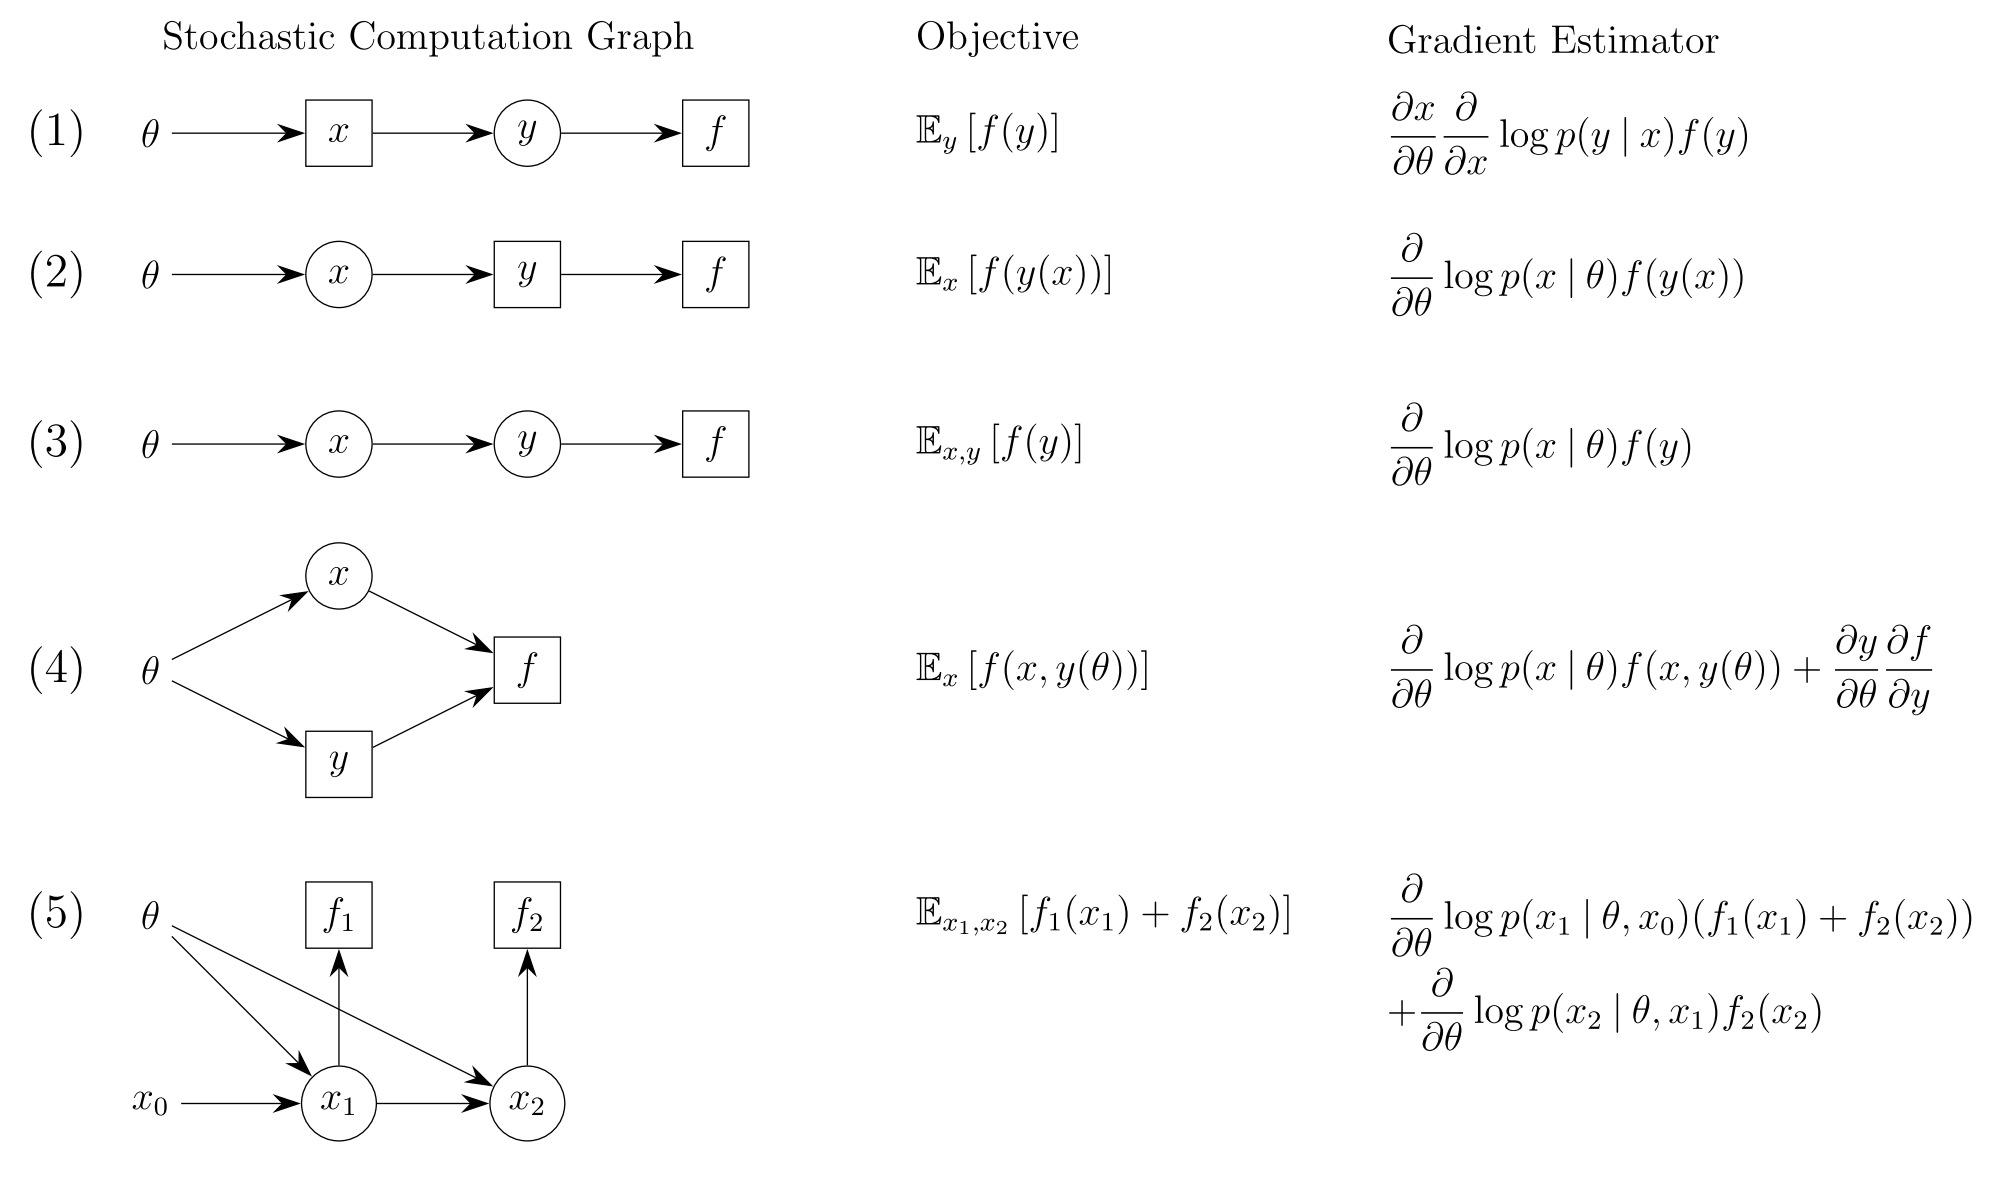
\includegraphics[width=\textwidth]{images/SCGs}
\caption[Stochastic Computation Graphs]{Simple examples of stochastic computation graphs (SCGs), along with the objective and corresponding gradient estimator. Nodes in circles are stochastic, nodes in squares are deterministic, and the rest are input nodes. Diagrams from \citet{schulman2015backprop}.}
\label{fig:scg}
\end{figure}

Figure~\ref{fig:scg} shows examples of simple SCGs, along with their corresponding objectives. To optimize the objective, we want to perform gradient descent, and so for any parameter $\theta$, we need to derive an estimator of its gradient.

We see in these special cases that there is an intuitive pattern to the gradient estimators. If there is a path from $\theta$ to the objective that goes through a stochastic node, we get a term for the derivative of the log probability multiplied by the objective. For paths through deterministic nodes, we get standard derivatives as in the chain rule from backpropagation.

Next, we derive the gradient of the objective with respect to parameter input nodes in the general case.

\section{Deriving the Gradients}

We define for nodes $w,v$ the relation $w \prec v$ (pronounced ``$w$ influences $v$'') if there exists a path from $w$ to $v$ in the SCG. We also say $w \prec^D v$ (``$w$ deterministically influences $v$'') if there exists a path that consists of only deterministic nodes.

Given an SCG, let $\mcS$ be the set of stochastic nodes and $\mcC$ the set of objective or cost nodes. For a given node $v$, let $\on{par}(v)$ denote its parents.

For a given parameter $\theta$, we have the following:
\begin{theorem}
Assume differentiability of all functions. Then the gradient of the objective with respect to $\theta$ is
\begin{align}
\frac{\partial}{\partial \theta} \mathbb{E}\left[ \sum_{c \in \mcC} \hat{c} \right] &= \mathbb{E}\left[\sum_{c \in \mcC} \hat{c} \sum_{v \in \mcS,~\theta \prec^D v, ~v \prec c }  \frac{\partial}{\partial\theta} \log p(v | \on{par}(v) ; \theta )  +
 \sum_{c\in \mcC,~\theta \prec^D c} \frac{\partial}{\partial \theta} \hat{c}
\right] \label{eq:gradient1} \\
&=  \mathbb{E}\left[ \sum_{v \in \mcS,~\theta \prec^D v} \left( \frac{\partial}{\partial\theta} \log p(v | \on{par}(v) ; \theta ) \right) \hat{C}_v + \sum_{c\in \mcC,~\theta \prec^D c} \frac{\partial}{\partial \theta} \hat{c} \label{eq:gradient2}
\right] 
\end{align}
where $\hat{C}_v = \sum_{c \in \mcC, ~v \prec c} \hat{c}$ is a random variable of the cost that stochastic node $v$ influences.
\label{thm:gradient}
\end{theorem}
Before we give the proof, we note the intuition. The first term represents the gradient from the stochastic nodes, where we multiply the gradient of the log probability with the cost.
The second term is the standard gradient we obtain from backpropagation, summed over all cost nodes that $\theta$ deterministically influences.
\begin{proof}
Due to linearity of expectation, we only need consider a single node $c \in \mcC$. Let $\mcL = \mathbb{E}[\hat{c}]$ be the loss function.

We have stochastic nodes $v$ such that $\theta \prec^D v$ and $v \prec c$, i.e. there is a path from $\theta$ to $c$ through $v$. Let this set be $\mcS_\theta$, and denote the joint random variable of this set as $\hat{\boldv}$. Let $c(\hat{\boldv} ; \theta)$ explicitly denote $\hat{c}$.

We compute the gradient:
\begin{align*}
\frac{\partial }{\partial \theta}\mathbb{E}[\hat{c}] &= \frac{\partial}{\partial \theta} \sum_{\hat{\boldv}} p(\hat{\boldv} | \on{par}(\boldv); \theta) \cdot c(\hat{\boldv}; \theta) \\
& = \sum_{\hat{\boldv}} \frac{ \partial  p(\hat{\boldv} | \on{par}(\boldv); \theta) } {\partial \theta} \cdot c(\hat{\boldv} ; \theta) + p(\hat{\boldv} | \on{par}(\boldv); \theta) \cdot \frac{\partial}{\partial\theta} c(\hat{\boldv}; \theta) \\
&= \sum_{\hat{\boldv}} \frac{ \partial  p(\hat{\boldv} | \on{par}(\boldv); \theta) } {\partial \theta} \cdot c(\hat{\boldv} ; \theta) + \mathbb{E}_{\boldv}\left[ \frac{\partial}{\partial\theta} c(\hat{\boldv}; \theta)  \right]
\end{align*}
Note that the second term gives the standard backpropagation gradient. We can rewrite the first term:
\begin{align*}
\sum_{\hat{\boldv}} \frac{ \partial  p(\hat{\boldv} | \on{par}(\boldv); \theta) } {\partial \theta} \cdot c(\hat{\boldv} ; \theta)
&= \sum_{\hat{\boldv}} p(\hat{\boldv} | \on{par}(\boldv); \theta) \frac{1}{p(\hat{\boldv}|\on{par}(\boldv);\theta)}\frac{ \partial  p(\hat{\boldv} | \on{par}(\boldv); \theta) } {\partial \theta} \cdot c(\hat{\boldv}; \theta) \\
&= \sum_{\hat{\boldv}} p(\hat{\boldv} | \on{par}(\boldv); \theta) \frac{ \partial  \log p(\hat{\boldv} | \on{par}(\boldv); \theta) } {\partial \theta} \cdot c(\hat{\boldv}; \theta) \\
 &= \mathbb{E}_{\hat{\boldv} \sim p(\hat{\boldv} | \on{par}(\boldv); \theta)} \left[ \frac{ \partial  \log p(\hat{\boldv} | \on{par}(\boldv); \theta) } {\partial \theta} \cdot c(\hat{\boldv} ; \theta) \right] \\
&= \mathbb{E}\left[ \widehat{c} \cdot \sum_{v \in \mcS_\theta} \frac{  \partial  \log p(\hat{v} | \on{par}(v); \theta) } {\partial \theta}  \right]
\end{align*}
where the last equality follows from separating the log joint probability term into its conditional marginals.

We have thus shown Equation~\ref{eq:gradient1}. Equation~\ref{eq:gradient2} follows directly by rearranging the order of summations, noting which nodes $v$ influence a certain $c$.

\end{proof}

Because the expectations in both gradient formulae are intractable in the general case, we use a single Monte Carlo sample as our gradient estimator.
This estimator is unbiased; however, the variance of the Monte Carlo gradient can be very high in practice.

%The training problem can be formalized as an RL problem. We can treat a neural network as a stochastic agent, and its computation serves to define the parametrized policy function $\pi(\cdot; w) : \mcS \to \mcA$.
%The states $\mcS$ are the inputs and the actions $\mcA$ are the possible outputs of each stochastic unit. The rewards are then negative loss (e.g. from regression or classification).


One of the simplest ways to reduce the variance of the gradient estimator is to introduce a baseline scalar $b \approx \mathbb{E}[\hat{c}]$ which we subtract from each cost term. That is, we have:
\begin{theorem}
The gradient of Equation~\ref{eq:gradient1} from Theorem~\ref{thm:gradient} can also be written as
\begin{equation}
\label{eq:baseline_gradient}
\frac{\partial}{\partial \theta} \mathbb{E}\left[ \sum_{c \in \mcC} \hat{c} \right] = \mathbb{E}\left[\sum_{c \in \mcC} (\hat{c} - b_c) \sum_{v \in \mcS,~\theta \prec^D v, ~v \prec c }  \frac{\partial}{\partial\theta} \log p(v | \on{par}(v) ; \theta )  +
 \sum_{c\in \mcC,~\theta \prec^D c} \frac{\partial}{\partial \theta} \hat{c}
\right] 
\end{equation}
where $b_c$ is a scalar not influenced by any of the $v$ in the summation.
\end{theorem}

\begin{proof}
Equation~\ref{eq:baseline_gradient} is identical to Equation~\ref{eq:gradient1}, except for the added terms
$$\mathbb{E}\left[ b_c \sum_{v\in \mcS, \theta \prec^D v, v \prec c}\frac{\partial}{\partial\theta} \log p(v | \on{par}(v) ; \theta) \right]$$
Considering a single $c$, by linearity it suffices to show that
\begin{equation*}
\mathbb{E} \left[ \frac{\partial}{\partial\theta} \log p(v | \on{par}(v) ; \theta) \right] = 0, \qquad \forall v \in \mcS_\theta
\end{equation*}
This is true since the $b_c$ term is constant with respect to the expectation (by our assumption that no $v$ influences it).

But this follows since
\begin{align*}
\mathbb{E} \left[ \frac{\partial}{\partial \theta} \log p(\hat{v} | \on{par}(v); \theta) \right] &= \sum_{\hat{v}} p(\hat{v} | \on{par}(v); \theta) \frac{\partial \log p(\hat{v} | \on{par}(v); \theta)}{\partial \theta} \\
&=  \sum_{\hat{v}} p(\hat{v} | \on{par}(v); \theta) \frac{1}{p(\hat{v} | \on{par}(v); \theta)} \frac{\partial  p(\hat{v} | \on{par}(v); \theta)}{\partial \theta}  \\
&= \frac{\partial}{\partial \theta} \sum_{\hat{v}} p(\hat{v} | \on{par}(v); \theta) =  \frac{\partial}{\partial \theta} [1] = 0
\end{align*}
Thus, the gradient with baseline is unbiased.
\end{proof}

Including a baseline is proven to reduce the variance of the estimator \citep{Weaver2001}. There are several different methods for producing baselines, such as taking the average of all previously seen cost terms, and we will not cover all of them here.

\section{Training}
\label{sec:algorithm}

In order to compute the gradients of SCGs in practice, we make a slight tweak to the backpropagation algorithm.

We first perform a forward pass of the SCG to obtain all values and samples for each node. In the backward pass, gradients for nodes that are directly connected to the cost nodes can be computed with usual backpropagation. For stochastic nodes, we first compute the costs $\hat{C}_v$ for node $v$ in Equation~\ref{eq:gradient2}. Broadcasting these values to the corresponding nodes, we can then continue backpropagation from the stochastic nodes with the gradient of the log probability.

Finally, if $g_\theta$ is the resulting gradient for parameter $\theta$, our gradient descent update is
\begin{equation}
\theta \gets \theta  - \eta g_\theta
\end{equation}
where $\eta$ is a learning rate.

Algorithm~\ref{alg:reinforce} gives the complete algorithm for gradient descent on SCGs.

Note that the resulting algorithm can easily be implemented in standard autodifferentiation packages for neural networks (e.g. Tensorflow, Torch). We only need to broadcast the costs $\hat{C}_v$ to each stochastic node, and implement the gradients accordingly.



\begin{algorithm}[t]
\caption{Gradient Descent for SCGs}
\label{alg:reinforce}
\begin{algorithmic}
\State Forward pass through SCG
\ForAll{$c \in \mcC$}
\State $\hat{c} \gets \hat{c} - b_c$ \Comment{Subtract baselines from costs}
\EndFor
\ForAll{$v \in \text{SCG}$}
\State $\boldg_v = \begin{cases} 1 & \text{if $v \in \mcC$} \\ 0 & \text{else} \end{cases}$
\State Compute $\hat{C}_v \gets \sum_{c \in \mcC, ~v \prec c} \hat{c}$ \Comment{Aggregated costs}
\EndFor

\For{$v$ in \textsc{ReverseTopologicalOrder}(SCG)} \Comment{Backpropagation}
\For{$w \in \on{par}(v)$}
\If{\textbf{not} \textsc{IsStochastic}($w$)}
\If{\textsc{IsStochastic}($v$)}
	\State $\boldg_w \text{ += } \hat{C}_w \cdot \frac{\partial}{\partial w} \log p(v | \on{par}(v) ) $
\Else
	\State $\boldg_w \text{ += } (\frac{\partial v}{\partial w})^\top \boldg_v$
\EndIf
\EndIf
\EndFor
\EndFor
\ForAll{parameters $\theta$}
\State $\theta \gets \theta - \eta g_\theta$ \Comment{Gradient descent}
\EndFor
\end{algorithmic}
\end{algorithm}


%Our policy gradient update from equation~\ref{eq:reinforce1} can therefore be summarized as
%\begin{equation}
%w^{(t+1)} \gets w^{(t)} + \eta \mathbb{E}_{a_t} \left[ (R_t - b) \frac{\partial \log p(a_t | s_t; w)}{\partial w} \right]
%\end{equation}




\section{Relation to Our Models}

Now that we understand the general definition of SCGs, we briefly overview how we will use them.


In the NLP problems we are interested in, we have a sequential decision problem as in reinforcement learning. That is, we have a trajectory of states $s_t$ and we make actions $a_t$ at time $t$ based on some parameterized policy function. Each action leads to a reward $r_t$ and determines our next state $s_{t+1}$, thus influencing total future reward $\sum_{s=t}^T r_s$ for finite $T$. See Figure~\ref{fig:our_scg} for a diagram.

\begin{figure}[t]
\begin{center}
\begin{tikzpicture}
        \node at (0,0) [rectangle,draw] (st) {$s_t$};
        \node at (3,0) [rectangle,draw] (stt) {$s_{t+1}$};
        \node at (6,0) [rectangle,draw] (sttt) {$s_{t+2}$};
	\coordinate  (st4) at (7,0) ;
	\coordinate  (st0) at (-1,0) ;

	\node at (-3,3)  (dots) {$\cdots$};
        \node at (0,3) [circle,draw] (at) {$a_t$};
        \node at (3,3) [circle,draw] (att) {$a_{t+1}$};
        \node at (6,3) [circle,draw] (attt) {$a_{t+2}$};
	\node at (9,3)  (dots) {$\cdots$};


	 \node at (0,5) [rectangle, draw] (rt) {$r_t$};
        \node at (3,5) [rectangle, draw] (rtt) {$r_{t+1}$};
        \node at (6,5) [rectangle, draw] (rttt) {$r_{t+2}$};

        \draw [->] (st) edge (stt);
	\draw [->] (stt) edge (sttt);
	\draw [->] (sttt) edge (st4);
	\draw [->] (st0) edge (st);

     \draw [->] (st) edge (at);
     \draw [->] (stt) edge (att);
     \draw [->] (sttt) edge (attt);
     \draw [->] (at) edge (rt);
     \draw [->] (att) edge (rtt);
     \draw [->] (attt) edge (rttt);
     \draw [dashed, ->] (at) edge (stt);
     \draw [dashed, ->] (att) edge (sttt);
    \end{tikzpicture}
\end{center}

\caption[Seq2Seq SCG]{The seq2seq SCG: the general form of the stochastic computation graph that appears in our problems. The squares nodes (states $s_t$) are deterministic hidden states, the circular nodes (actions $a_t$) are stochastic, and $r_t$ comes from our training loss. Our graph is abbreviated --- each arrow can potentially have many intermediate nodes and parameters. }
\label{fig:our_scg}
\end{figure}

The resulting SCG will turn out to mirror the computation graph for sequence-to-sequence models with attention. There, $s_t$ will be the hidden state of our model when generating word $t$, and $r_t$ comes from our loss function during training. In that case, the stochasticity of $a_t$ can arise from a mechanism such as hard attention.


With this setup in mind, we describe our models in detail in the next chapter.

%, we are interested to see if the same  can be applied to the document summarization problem. We will introduce stochastic nodes into a deep learning model and investigate the feasibility of using policy gradient methods for conditional computation.
%
%In the next chapter we describe our models in detail.
%

% Note that we can treat our actions $a_t$ for $ t = 0, \ldots, T$ as stochastic nodes in an SCG, and the costs $\hat{c}$ are the rewards we receive for each $t$. Then instead of computing $\hat{C}_{a_t} = \sum_{s=t}^T r_s$, we can scale later rewards with a discount factor $\gamma $, giving
%\begin{equation}
%\hat{C}_{a_t} = \sum_{s=t}^T \gamma^{s-t} r_s
%\end{equation}
%which fits neatly in with Algorithm~\ref{alg:reinforce}. We will use this RL setup to discuss our models, and our algorithms are confidently backed up by the theory of SCGs.
%
%Even before the concept of SCGs were formalized, reinforcement learning and deep learning have successfully been combined to play Go \citep{Silver2016}, 
%control robots \citep{Levine2016}, and play Atari games from pixels \citep{deepatari2015}.
%In computer vision, policy gradient methods have been fairly successful on several tasks
%\citep{mnih2014visualattention, ba2015visualattention, xu2015captioning}.
%In NLP, reinforcement learning research is still preliminary, but has been attempted with varying degrees of success so far.
%\citet{ranzato2015} apply RL to improve sequential estimation by e.g. training on BLEU rewards for machine translation.
%\citet{Narasimhan2015} use RL play text-based games.
%\citet{li2016dialogueRL} use RL to train an end-to-end dialogue system.
%\citet{narasimhan2016} use RL to improve information extraction on scarce data.
%%\citet{Andreas2016} uses RL to compose 
%\citet{Yogatama2017} use RL along with an architecture called a tree LSTM that produces a tree-structured latent variable on a sentence using \textsc{Shift} and \textsc{Reduce} actions. They show that the tree LSTM can produce reasonable parse structures by solely using RL methods.
%
%In computer vision, this SCG has been used successful on several tasks
%\citep{mnih2014visualattention, ba2015visualattention, xu2015captioning}.

\chapter{Models}
\label{chap:models}

In this chapter, we describe our models. We begin by introducing the standard sequence-to-sequence attention model, then describe our extensions of the basic architecture.

\section{Sequence-to-sequence (seq2seq)}

We first describe the neural network architecture of the seq2seq models, also known as encoder-decoder models \citep{bahdanau2014neural}.


In the seq2seq model, an \emph{encoder} recurrent neural network (RNN) reads the source sequence as input to produce the \emph{context}, and a \emph{decoder} RNN generates the output sequence using the context as input.  One popular RNN choice is the long-short term memory (LSTM) network \citep{hochreiter1997long}.

\begin{figure}[t]
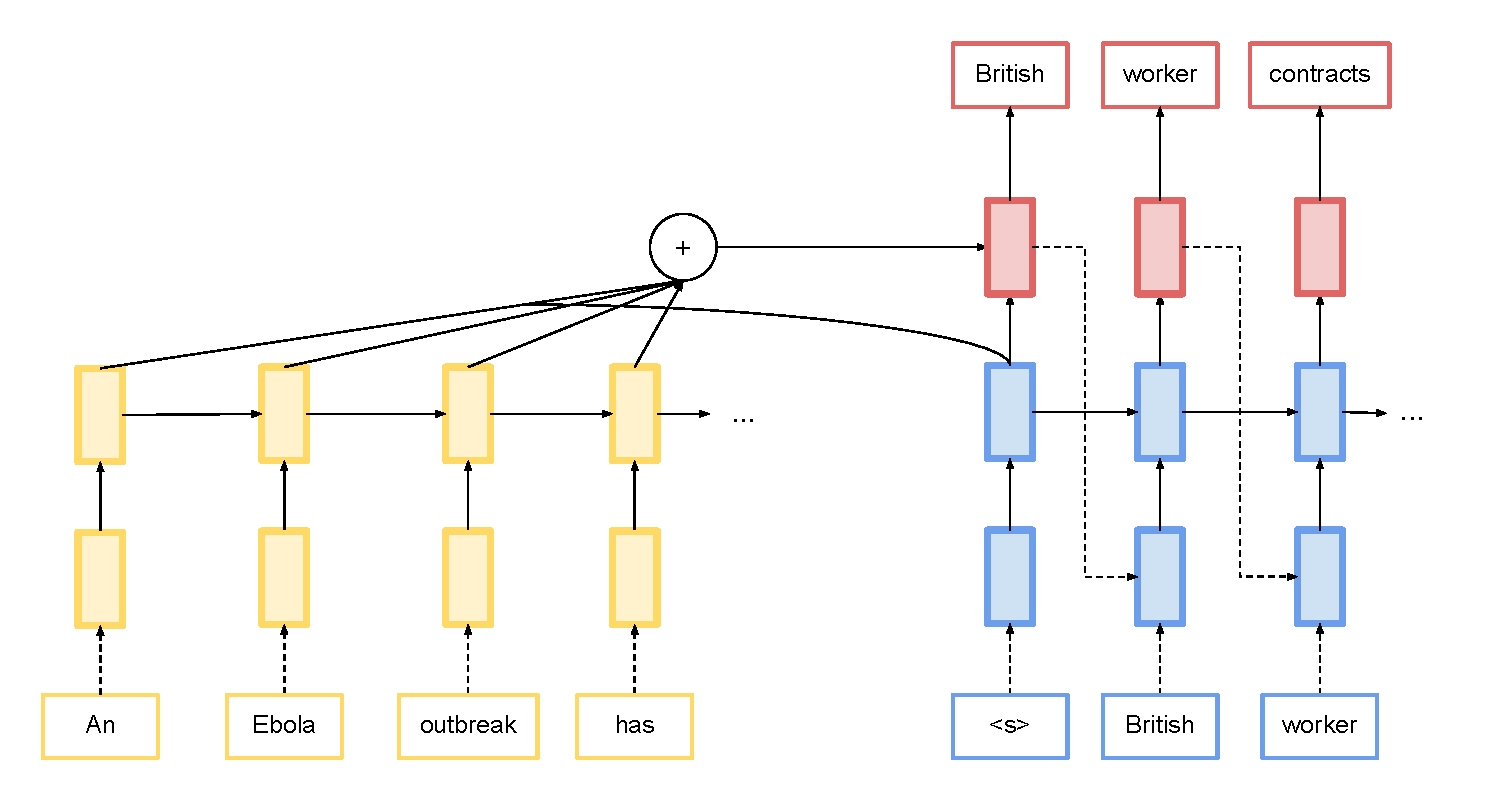
\includegraphics[width=\textwidth]{images/seq2seq}
\caption[Sequence-to-Sequence Model]{Model architecture for sequence-to-sequence with attention, or \textsc{Model 0}. The yellow hidden states are the encoder, the blue hidden states are the decoder, and the red hidden states are the generator. The decoder hidden state at each time step determines the attention weights, which we use to average the encoder hidden states to produce a context vector. The result feeds into the generator.}
\label{fig:seq2seq}
\end{figure}


More formally, suppose we have a vocabulary $\mcV$. A given input sentence $w_1, \ldots, w_n \in \mathcal{V}$ is transformed into a sequence of vectors $\boldx_1, \ldots, \boldx_n \in \mathbb{R}^{d_{in}}$ through a word embedding matrix $\boldE \in \mathbb{R}^{|\mathcal{V}| \times d_{in}}$ as $\boldx_t = \boldE w_t$.

An RNN is given by a parametrizable function $f_{enc}$ and a hidden state $\boldh_t \in \mathbb{R}^{ d_{hid}}$ at each time step $t$ with $\boldh_t = f_{enc}(\boldx_t, \boldh_{t-1})$. For the LSTM, we keep an auxiliary state $\boldc_t$ along with $\boldh_t$, and we compute $f_{enc}$ as
\begin{align}
\boldf_t &= \sigma(\boldW^f \boldx_t + \boldU^f \boldh_t + b_f) \\
\boldi_t &= \sigma(\boldW^i \boldx_t + \boldU^i \boldh_t + b_i) \\
\boldo_t &= \sigma(\boldW^o \boldx_t + \boldU^o \boldh_t + b_o) \\
\boldc_t &= \boldf_t \odot \boldc_{t-1}  + \boldi_t \odot \tanh(\boldW^c \boldx_t + \boldU^c \boldh_{t-1} + b_c) \\
\boldh_t &= \boldo_t \odot \tanh(\boldc_t)
\end{align}
where $\boldW, \boldU, b$ are learned parameters, $\sigma$ is the sigmoid function, and $\odot$ is the elementwise product. 
Intuitively, $\boldc_t$ is the memory cell, $\boldf_t$ is the forget gate, $\boldi_t$ is the input gate, $\boldh_t$ is the output cell, and $\boldo_t$ is the output gate.

LSTMs can be stacked on top of one another by treating the outputs $\boldh_t$ of one LSTM as the inputs to another LSTM. In stacked LSTMs, we will take the top sequence of hidden states $\boldh_1, \ldots, \boldh_n$ to form the context hidden states.


The decoder is another RNN $f_{dec}$ that generates output words $y_t \in \mathcal{V}$. It keeps hidden state $\boldh_t^{dec} \in \mathbb{R}^{d_{hid}}$ as $\boldh_t^{dec} = f_{dec}(y_{t-1}, \boldh_{t-1}^{dec})$ similar to the encoder RNN.
A context vector is produced at each time step using an attention function $a$ that takes the encoded hidden states $[\boldh_1, \ldots, \boldh_n]$ and the current decoder hidden state $\boldh_t^{dec}$ and produces the context $\boldc_t \in \reals^{d_{ctx}}$:
\begin{equation}
\boldc_t = a([\boldh_1, \ldots, \boldh_n], \boldh_t^{dec})
\end{equation}
As in \citet{luong2015effective}, it is helpful to feed the context vector at time $t-1$ back into the decoder RNN at time $t$, i.e. $\boldh_t^{dec} = f_{dec}([y_{t-1}, \boldc_{t-1}], \boldh_{t-1}^{dec})$.

Finally, a linear projection produces a distribution over output words $y_t \in \mcV$:
\begin{equation}
p(y_t | y_{t-1}, \ldots, y_1, [h_1, \ldots, h_n]) = \boldW^{out}\boldc_t + b^{out}
\end{equation}

Given document-summary pairs $\{ (\boldx^{(i)}, \boldy^{(i)}) \}_{i=1}^N$ for training, the models are trained to maximize the log probability of getting the sequences in the dataset correct, i.e. minimize the negative log-likelihood (NLL):
\begin{align*}
\mcL(\theta) &= - \sum_{i=1}^N \log p(\boldy^{(i)} | \boldx^{(i)}; \theta)  \\
&= -\sum_{i=1}^N \sum_{t=1}^{T-1} \log p(y_{t+1}^{(i)} | \boldx^{(i)}, y_t^{(i)}, \ldots, y_1^{(i)} ; \theta)
\end{align*}
As the model is fully differentiable with respect to its parameters, we can train it end-to-end with stochastic gradient descent and the backpropagation algorithm.

We note that we have great flexibility in how our attention function $a(\cdot)$ combines the encoder context and the current decoder hidden state. In the next few sections, we explain standard choices for $a(\cdot)$ as well as our proposed model of coarse-to-fine attention.

\section{Model 0: Standard Attention}

In \citet{bahdanau2014neural}, the function $a(\cdot)$ is implemented with an \emph{attention network}. We compute attention weights for each encoder hidden state $h_i$ as follows:
\begin{align}
\beta_{t,i} &= \boldh_i^\top \boldW^{attn} \boldh_t^{dec} \quad \forall i = 1, \ldots, n\\
\balpha_t &= \mathrm{softmax}(\bbeta_t) \\
\widetilde{\boldc}_t &= \sum_{i=1}^n \alpha_{t,i} \boldh_i
\end{align}
The idea behind attention is to select the most relevant words of the source (by assigning higher attention weights) when generating output word $y_t$ at time $t$.

The $\mathrm{softmax}$ function, defined as
\begin{equation}
\mathrm{softmax}([\beta_1, \ldots, \beta_n])_i =  \frac{\exp(\beta_i)}{\sum_{j=1}^n \exp(\beta_j)}
\end{equation}
normalizes the $\alpha_i$ to sum to 1 over the source sentence words. This gives us a notion of probability distribution over the encoder words --- we can therefore write $\boldc_t$ as the expectation $\mathbb{E}_\alpha[\boldh]$, where we pick $\boldh_i$ with probability $\alpha_i$.

Our final context vector is then
\begin{equation}
\boldc_t = \tanh(\boldW^2[\widetilde{\boldc}_t, \boldh_t^{dec}])
\end{equation}
for $\boldW^2 \in \reals^{2d_{hid} \times d_{ctx}}$ a learned matrix.

Going forward, we call this instantiation of the attention function \textsc{Model 0}.


\section{Model 1 and 2: Coarse-to-Fine Soft Attention}

\begin{figure}
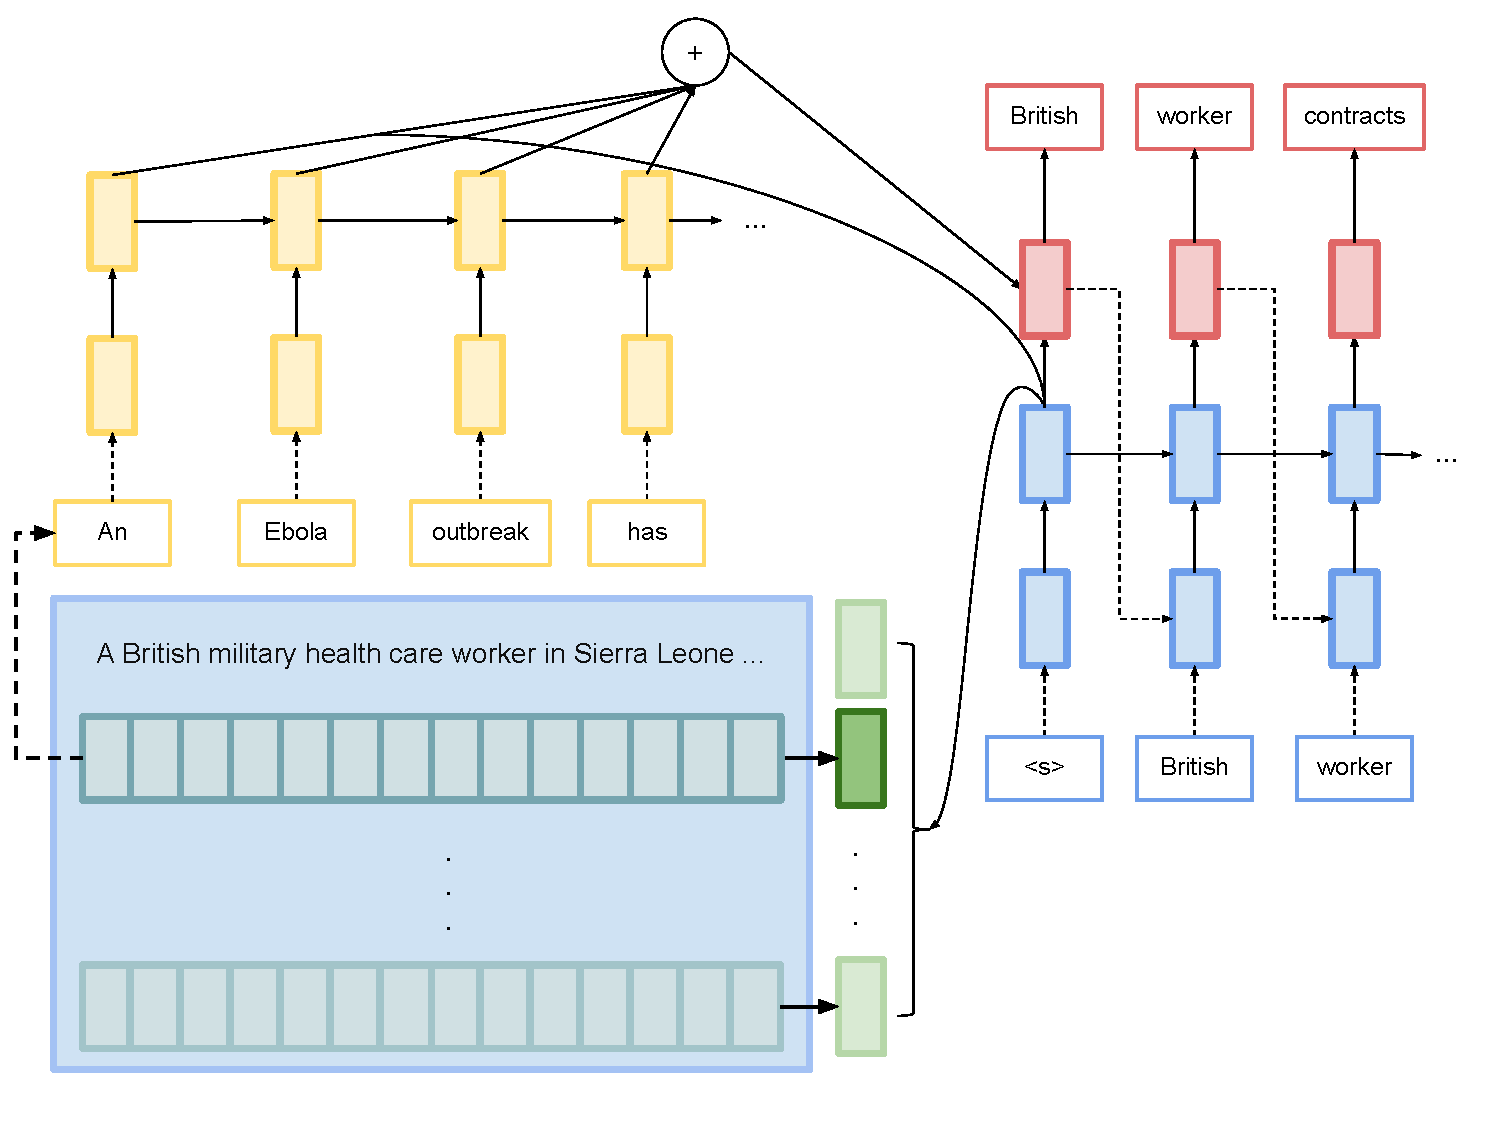
\includegraphics[width=\textwidth]{images/coarse_to_fine.pdf}
\caption[Coarse-to-Fine Attention Model]{Model architecture for sequence-to-sequence with coarse-to-fine attention. The left side is the encoder that reads the document, and the right side is the decoder that produces the output sequence. On the encoder side, the green hidden states (sentence-level) are used for the coarse attention weights, while the yellow hidden states (word-level) are used for the fine attention weights. The context vector is then produced by averaging the word-level states. In \textsc{Model 2}, we average over the coarse attention weights, thus requiring computation of all word-level hidden states. In \textsc{Model 3}, we make a hard decision for which sentence to use, and so we only need to compute word-level hidden states for one sentence.}
\label{fig:coarsetofine}
\end{figure}

The attention network of \textsc{Model 0} is computationally expensive for long sentences --- for each hidden state of the decoder, we need to compare it to every hidden state of the encoder in order to determine where to attend to.
This seems unnecessary for a problem such as document summarization; intuitively, we only need to attend to a few important sentences at a time. Therefore, we propose a hierarchical method of attending to the document by first attending to sentences, then to the words within sentences. We call this method \emph{coarse-to-fine attention}\footnote{The term coarse-to-fine attention has previously been introduced in the literature \citep{mei2016}. However, their idea is different: they use coarse attention to reweight the fine attention computed over the entire input. This idea has also been called hierarchical attention \citep{nallapati2016seq2seq}.}.



To be able to attend to both sentences and words in a hierarchical manner, we need to construct encodings of the document at both levels. For the coarse-grained sentence representations, we use a simple encoding model (e.g. bag of words), and for the fine-grained representations, we run an LSTM encoder on the words of a sentence.
Thinking about text at different levels of granularity is motivated by \citet{li2015autoencoder}, who use the idea of a hierarchical representation of text to develop an autoencoder for paragraph representation.

%\citet{Sukhbaatar2015} demonstrate how coarse representations can be useful by using memory networks to access information for simple question-answering tasks.
%by using low-level LSTMs on words to build sentence representations, then a high-level LSTM on the sentences for the final paragraph representation.

Therefore, if we can make our model first use coarse attention to choose sentences, then use fine attention to choose words only from that sentence, then we avoid the computational cost of searching over the entire document.

Specifically, suppose we have sentences $s_1, \ldots, s_m$ with words $w_{i,1}, \ldots, w_{i,n_i}$ for sentence $s_i$. We apply an RNN to each sentence separately to get corresponding hidden states $\boldh_{i,j}$ for $i = 1, \ldots, m$ and $j = 1, \ldots, n_i$, so that
\begin{equation}
\boldh_{i,j} = \on{RNN}(\boldh_{i,j-1}, w_{i,j})
\end{equation}
For attention, we then consider two options.

\paragraph{Model 1} We can follow \textsc{Model 0} and compute attention weights $\alpha_{i,j}$ for each hidden state $\boldh_{i,j}$ by normalizing over all states.
This is a slightly weakened version of \textsc{Model 0}; like \textsc{Model 0}, we normalize attention over all hidden states at once, but now our RNN hidden states do not share context between sentences. We call this \textsc{Model 1}.

\paragraph{Model 2} Alternatively, rather than taking attention over the entire document, we can instead have a two-layered hierarchical attention mechanism: first, we have weights $\alpha_1^s, \ldots, \alpha_m^s$ for each sentence, and then for sentence $s_i$, we have another set of weights $\alpha_{i,1}^w, \ldots, \alpha_{i,n_i}^w$.
Our final attention weight on word $w_{i,j}$ is then $\alpha_{i,j} = \alpha_i^s \cdot \alpha_{i,j}^w$.

In order to compute the sentence attention weights $\alpha_i^s$, we need to produce representations of each sentence; i.e., given the words $w_{i,1}, \ldots, w_{i, n_i}$ of the sentence, we produce a vector representation $\boldh^s_i \in \mathbb{R}^{d_{sent}}$. Figure~\ref{fig:sent_reps} shows diagrams of our sentence representation models.

\begin{figure}[t]
\centering
\begin{subfigure}{0.45\textwidth}
	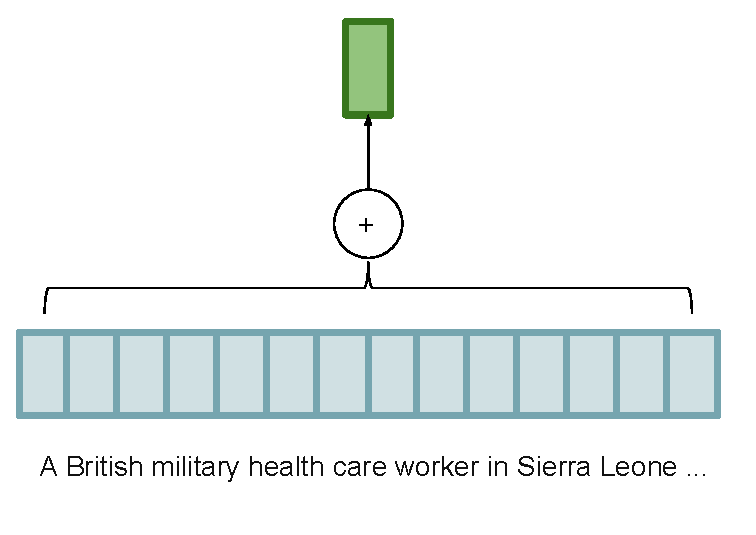
\includegraphics[width=\textwidth]{images/bow_encoder_bow}
  \caption[Bag of Words Encoder]{Bag-of-words}
	\label{fig:bow_encoder_bow}
\end{subfigure}
\begin{subfigure}{0.45\textwidth}
	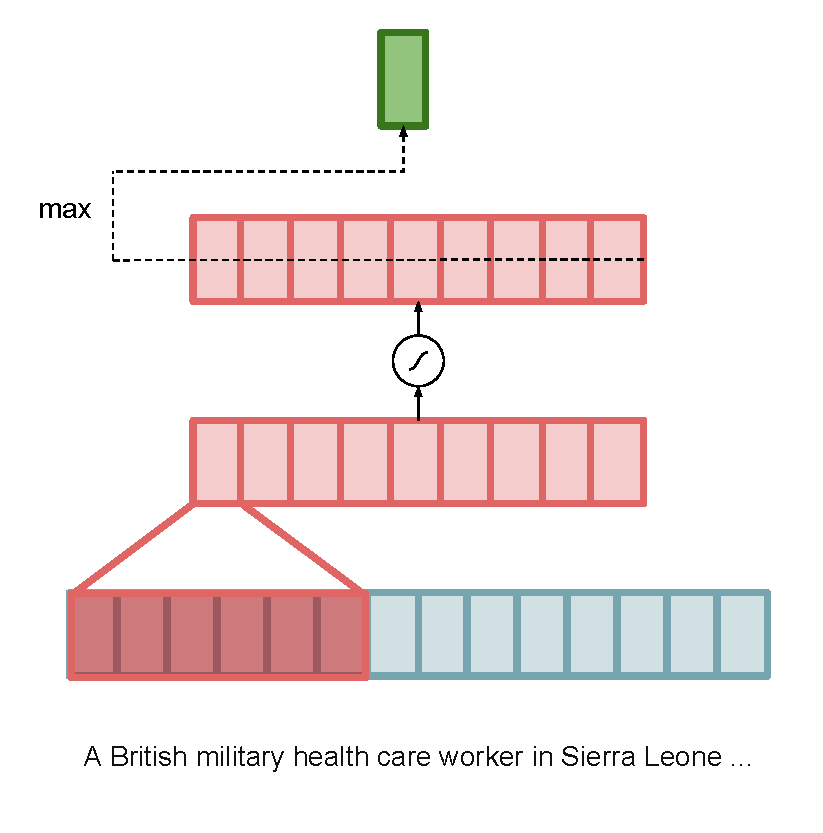
\includegraphics[width=\textwidth]{images/bow_encoder_conv}
  \caption[Convolutional Encoder]{Convolution}
	\label{fig:bow_encoder_conv}
\end{subfigure}
\caption[Sentence Representation Encoders]{Options for producing sentence representations from the word embeddings. We can either use a bag of words by summing the embeddings, or apply convolutions and max-over-time pooling. The output is a sentence representation in $\reals^{d_{sent}}$. }
\label{fig:sent_reps}
\end{figure}

Our first option is bag of words: we simply take the representation as
\begin{equation}
\boldh_i^s = \sum_{j=1}^{n_i} \boldE w_{i,j}
\end{equation}
i.e. the sum of the word embeddings, where $\boldE$ is another embedding matrix.

Alternatively, we can use a convolutional method: as in \citet{kim2014convolutional}, we perform a convolution over each window of words in the sentence using a fixed kernel width. We use max-over-time pooling to obtain a fixed-dimensional sentence representation in $\mathbb{R}^{d_f}$ where $d_f$ is the number of filters.

Explicitly, fix a sentence and suppose we have word vectors $\boldx_1, \ldots, \boldx_n$ with $\boldx_j = \boldE w_j \in \reals^{d_{in}}$, and suppose we have kernel width $k$ and convolution weights $\boldW^{conv} \in \reals^{d_f \times d_{in} k}$ where $d_f$ is the number of filters. Then applying the convolution
$\boldW^{conv} * [\boldx_1, \ldots, \boldx_n]$ gives result $\boldu = [\boldu_1, \ldots, \boldu_{n-k+1}]$ with $j$th element
$$\boldu_j = \boldW^{conv} \cdot [\boldx_j, \boldx_{j+1}, \ldots, \boldx_{j+k-1}] + \boldb^{conv} \in \reals^{d_f}$$
Our final output is given by 
\begin{equation}
\boldh^s = \max_j(\tanh(\boldu_j))
\end{equation}
where the max-over-time takes the maximum along the word indexing dimension.

As an addition to any sentence representation method, we can include \emph{positional embeddings}. In general, we expect the order of sentences in the document to matter for summarization --- for example, the first few sentences are usually important.
We therefore include the option to concatenate a small fixed-dimensional embedding of the sentence's position to the existing representation.

Thus, using the sentence representations, we can compute attention $\alpha_i^s$ over the sentences.
For the words in each sentence, we run an LSTM over each sentence separately, and create attention weights $\alpha_{i,j}^w$ over the words in each sentence in the same way as \textsc{Model 0}. Using attention on word $w_{i,j}$ as  $\alpha_{i,j} = \alpha_i^s \cdot \alpha_{i,j}^w$, we can proceed exactly as in \textsc{Model 0} by computing the weighted average over hidden states $\boldh_{i,j}$.

We call this method of attention \textsc{Model 2}.

\section{Model 3: Coarse-to-Fine Sparse Attention}

With the previous models, we are required to compute hidden states over all words and sentences in the document, so that if we have $M$ sentences and $N$ words per sentence, the computational complexity is $O(MN)$ for each attention step.

However, if we are able to perform conditional computation and only compute on $M^+$ of the sentences, we can reduce the complexity to $O(M^+N)$. If we are able to make $M^+$ constant or even 1, the complexity of attention becomes $O(N)$ --- an expression invariant of the length of the document!

In our experiments, we will apply stochastic sampling to the attention distribution $\balpha$ in the spirit of ``hard attention'' \citep{xu2015captioning}.
Specifically, rather than computing the context $\widetilde{\boldc}$ as an expectation over $\balpha$ (i.e. $\widetilde{\boldc} = \sum_{i=1}^n \alpha_i \boldh_i$), we can sample from the probability distribution $\balpha$ to obtain a single state $\boldh_i$, and we set $\widetilde{\boldc} = \boldh_i$ as the sampled hidden state.

In our case, we take \textsc{Model 2} and apply hard attention at the sentence level, but keep the word level attention per sentence as is. That is, we sample from the attention weights $\alpha_1^s, \ldots, \alpha_m^s$ to obtain a one-hot encoding for the sentence attention, and apply the same multiplication with this one-hot vector on the word-level attention weights $\alpha_{i,1}^w, \ldots, \alpha_{i,n_i}^w$ for all $i = 1, \ldots, m$. At test time, we take the max $\alpha_i^s$ for our one-hot encoding instead of sampling. We call this \textsc{Model 3}.


Because the hard attention model loses the property of being end-to-end differentiable, we use reinforcement learning to train our network.


\subsection{Practical Considerations}
\label{sec:practical}

Our hard attention model is now a stochastic computation graph, and thus Algorithm~\ref{alg:reinforce} from Section~\ref{sec:algorithm} applies.

Here, we have an RL agent where the state $s_t$ is the LSTM decoder state at time $t$, and actions $a_t$ are the hard attention decisions.
Since samples from $\balpha_t$ at time $t$ of the RNN decoder can also affect future rewards, in the notation of Chapter~\ref{chap:algorithms}, the total influenced reward is $\hat{C}_t = \sum_{s = t}^T r_s$ at time $t$, where $r_t = \log p(y_t | y_1, \ldots, y_{t-1}, \boldx)$ is the single step reward.

Inspired by the discount factor from RL, we slightly modify the total reward: instead of simply taking the sum, we can scale later rewards with a discount factor $\gamma $, giving
\begin{equation}
\hat{C}_{a_t} = \sum_{s=t}^T \gamma^{s-t} r_s
\end{equation}
for the stochastic hard attention node $a_t$. We found that adding a discount factor helps in practice (we use $\gamma = 0.5$).
%which fits neatly in with Algorithm~\ref{alg:reinforce}. We will use this RL setup to discuss our models, and our algorithms are confidently backed up by the theory of SCGs.

To calculate the baselines for variance reduction, we store a constant $b_t$ for each decoder time step $t$. We follow \citet{xu2015captioning} and keep an exponentially moving average of the reward for each time step $t$:
\begin{equation}
b_t \gets b_t + \beta (r_t - b_t)
\end{equation}
where $r_t$ is the average minibatch reward and $\beta$ is a learning rate (set to 0.1).

While several papers suggest using a learned baseline \citep[e.g.][]{mnih2014visualattention, ranzato2015}, we have not found this to be effective. In our experiments, we found that attempting to learn the baseline failed to converge, most likely because there is not enough correlation between the reward and the hidden states preceding the attention layer.

In addition to including a baseline, we also scale the rewards by a tuned hyperparameter --- we found that scaling helped to stabilize training. We empirically set the scale to 0.3.



%Similarly, we keep a moving average of the variance for normalization:
%$$\sigma^2_j = (1 - \beta) \sigma^2_{j-1} + \beta v_j$$
%where $v_t$ is the variance of the minibatch rewards for batch $j$. Since we have rewards at each time step of the decoder LSTM, we keep a separate moving average for the baseline for each time step, but we keep a single moving variance for all time steps.



\paragraph{\textsc{Alternate} training} \citet{xu2015captioning} explain that training hard attention with REINFORCE has very high variance, even when including a baseline. Thus, for every minibatch of training, they randomly use soft attention instead of hard attention with some probability (they use 0.5).
The backpropagated gradient is then the standard soft attention gradient instead of the REINFORCE gradient. In our results, we label this as \textsc{+alternate}.

While this method helps stabilize training, we would prefer not to use it. Our goal in coarse-to-fine attention is to reduce computation, but \textsc{alternate} training requires full attention computation for a subset of minibatches. However, this training method still allows for computational benefits at test time, and we include it in our experiments to test the feasibility of hard attention.


\paragraph{Multiple samples} 
From our initial experiments with \textsc{Model 3}, we found that taking a single sample was not very effective. However, we discovered that sampling multiple times from the attention distribution $\balpha^s$ improves performance.

To be precise, we fix a number $k_{mul}$ for the number of times we sample from $\balpha^s$. Then, we sample based on the multinomial distribution $\bmu \sim \mathrm{Mult}(k_{mul}, \{\alpha_i\}_{i=1}^m)$ to produce the new sentence-level attention vector $\widetilde{\balpha}^s$, with $\widetilde{\alpha}_i^s = \mu_i / k_{mul}$. In our results, we label this as \textsc{+multi}.

Intuitively, $k_{mul}$ is the number of sentences we select to produce the context. With higher $k_{mul}$, the hard attention model more closely approximates the soft attention model, and hence leads to better performance. This, however, incurs a cost in computational complexity.

%\section{Beam Search}
%
%Once we have our trained model, we use beam search at test time to produce the output summaries.
%
%In beam search, we keep a beam of $k$ hypotheses at every time step $t$. \todo{finish}
%
%\begin{algorithm}[b]
%\caption{Beam Search}
%\label{alg:beam_search}
%\begin{algorithmic}
%\State todo
%\end{algorithmic}
%\end{algorithm}



%We also include an entropy-increasing term to encourage exploration during the training process, which is important to speed up convergence of learning. Our policy gradient equation then becomes
%\begin{equation}
%w \gets w + (R_t - b) \frac{\partial \log p(\balpha_t | y_1, \ldots, y_{t-1})}{\partial w}
% + \lambda_{ent} \frac{\partial H(\balpha_t)}{\partial \balpha_t}
%\end{equation}
%where $H(\balpha_t) = -\sum_{i=1}^n \alpha_t \log \alpha_t$ is the entropy function and $\lambda_{ent}$ is a hyperparameter.



%\subsection{Curriculum}
%
%Since training using policy gradients tends to be noisy and slow to converge, we experimented with a curriculum that starts training with soft attention and in epoch $t$, trains a minibatch using hard attention with probability $p_t = 1 - 1/\sqrt{t}$ \citep{bengio2016hardntm}.
%
%While we found this to be helpful for single sample hard attention, it was not necessary for effective training with multisampled hard attention. We prefer to train solely with hard attention when possible, as we are able to save computation at training time.

%\section{Sparsemax}
%
%% describe


\chapter{Experiments}
\label{chap:experiments}

In this chapter, we describe our experimental setup.

\section{Data}

\subsection{CNN/Dailymail}

Experiments were performed on the CNN/Dailymail dataset from \cite{Hermann2015}.
While the dataset was created for a question-answering task, the dataset format is suited for summary. Each data point is a news document accompanied by up to 4 ``highlights'', and we take the first of these as our target summary.



Train, validation, and test splits are provided along with document tokenization and sentence splitting. We do additional preprocessing by replacing all numbers with \# and appending end of sentence tokens \texttt{<s>} to each sentence. We limit our vocabulary size to the 50000 most frequent words, replacing the rest with \texttt{<unk>} tokens. We dropped the documents which had an empty source (which came from photo articles).

 Table~\ref{table:data_stats} lists statistics for the CNN/Dailymail dataset. Figure~\ref{fig:data_examples} shows examples source and target pairs from the dataset.



% dataset statistics
\begin{table}[h]
\centering
\begin{tabular}{lccc}
\toprule
Dataset  & CNN & Dailymail & Combined\\
\midrule
Train size & 90266 & 196961 & 287227\\
Valid size & 1220 & 12148 & 13368\\
Test size & 1093 & 10397 & 11490 \\
Avg. \# words per doc. & 794 & 831 & 819\\
Avg. \# sent. per doc. & 21 & 29 & 26\\
Avg. \# words per sent. & 36 & 27 & 29\\
Avg. \# words per summary & 13 & 14 & 14\\
\bottomrule
\end{tabular}
\caption[CNN/Dailymail Statistics]{Statistics for CNN/Dailymail data. Numbers are collected over the training data.}
\label{table:data_stats}
\end{table}

\begin{figure}
\centering
\begin{tabular}{p{0.7\linewidth} r p{0.2\linewidth}}
\toprule 
\textbf{Document} & & \textbf{Summary} \\
\midrule 
( cnn ) the man suspected of killing a deputy u.s. marshal at a motel in baton rouge , louisiana , has died , brittany stewart in the east baton rouge coroner 's office said wednesday . \texttt{</s>} the cause of death is pending autopsy , she said . \texttt{</s>} jamie croom , \#\# , was wounded in a shootout with deputy u.s. marshal josie wells . \texttt{</s>} it can be one of the most dangerous tasks for a law enforcement officer : serving an arrest warrant to a fugitive murder suspect . when wells tried to do that tuesday , he lost his life . \texttt{</s>}  ... & & the fugitive who killed the marshal was " extremely dangerous , " u.s. marshals service director says \\
\midrule
( cnn ) there have been a few times in my career when i 've been thoroughly disappointed -- even disgusted -- with my fellow women in the workplace . \texttt{</s>} no , i certainly do n't expect all my female colleagues to go out of their way for me and sing " kumbaya " together in the office , but i 'm always stunned when a woman who could have been helpful to me was n't , when a woman who could have been a mentor chose not to be , when a woman tried to hurt me because of her own fear , anxiety or what have you . \texttt{</s>} i 'd love to say more about each of the women i 've met along the way who fit those descriptions , but my point is not to single anyone out . my goal is to ask the question , " why ? " \texttt{</s>} obviously , not all women are like this and there are plenty of men guilty of the same behavior , but why do so many women try to tear each other down instead of lift each other up ? \texttt{</s>} ... & & cnn 's kelly wallace wonders why women too often do n't lift each up in the workplace \\
\midrule
much of the start of the world 's most famous sled dog race is covered in barren gravel , forcing iditarod organizers to move the start further north where there is snow and ice . \texttt{</s>} a weather pattern that buried the eastern u.s. in snow has left alaska fairly warm and relatively snow - free this winter , especially south of the alaska range . \texttt{</s>} ' if i have one more person say to me to move the iditarod to boston , i 'm going to shake my head , ' said race director mark nordman . \texttt{</s>} scroll down for video in this photo taken on thursday , there are bare patches of grass and mud on sled dog trails in anchorage , alaska which is unsuitable for the iditarod \texttt{</s>}  ... & & much of the start of the world 's most famous sled dog , the iditarod trail sled dog race , is covered in barren gravel \\
%\midrule
%a store clerk manged to foil an armed robber with just the swat of his hand . \texttt{</s>} the workers , who was behind the counter at the ok food store in houston , texas early thursday
% morning , got the shock of his life when a young man pulled a gun on him and demanded money as he opened the register . \texttt{</s>} rather than hand over the bills however , the clerk , who is not being identified , started hitting at the man 's gun repeatedly , sending him and his accomplice running from the store . \texttt{</s>} scroll down for video a man 's attempt to rob a store in houston , texas was caught on video \texttt{</s>} the man entered the store and pretended to be a customer , being joined by a friend soon after \texttt{</s>} when the cashier opened the register the man pulled out a gun \texttt{</s>} the gunman first enters pretending to be a customer , pointing out things to the clerk as he takes out a large wad of cash . \texttt{</s>} then , a minute later , his friend leaves the car and joins him in the store . \texttt{</s>} when the clerk then opens up the cash register to make the sale , the gun comes out . \texttt{</s>} ... & & a man attempted to rob the ok food store in houston , texas early thursday morning at gunpoint \\
% \midrule
% ( cnn ) a michigan woman lost her planet fitness membership over the " inappropriate " manner in which she complained about a transgender woman in the locker room , a gym spokeswoman said . \texttt{</s>} yvette cormier 's membership was not canceled for simply raising the issue , " as we welcome all feedback from our members , " said mccall gosselin , director of public relations at planet fitness corporate . \texttt{</s>} rather , it was the manner in which she expressed her concerns that club management felt was inappropriate , resulting in the cancellation , gosselin said . \texttt{</s>} cormier stands by her actions in a case that has drawn attention to transgender rights . \texttt{</s>} " this is all new to me . i did n't go out to specifically bash a transgender person that day . i was taken aback by the situation , " cormier told cnn . " this is about me and how i felt unsafe . i should feel safe in there . " \texttt{</s>} the mother of two says she was acting out of concern for her safety and the privacy of other female gym members when she raised the issue on saturday , february \#\# . \texttt{</s>} ... & & woman loses gym membership after complaining about transgender woman in locker room \\
% \midrule

%( cnn ) the american civil liberties union is challenging an alabama law that will force those under \#\# seeking an abortion to go through an adversarial process that 's akin to a trial . \texttt{</s>} generally , laws in the united states require parental consent for a minor to obtain an abortion . but for some children , parental consent is impossible or even dangerous . this class of minors must seek a judicial bypass . while the bypass is a common feature of abortion laws in other states , this alabama law may have gone too far . here are the suspect provisions of this " bypass by trial " : \texttt{</s>} alabama has turned what is supposed to be an informal , child - centered hearing into more of a trial . \texttt{</s>} the court can appoint a guardian ad litem -- normally an appointed lawyer for a child in , say , a divorce proceeding or a hearing involving unfit parents -- for the fetus . \texttt{</s>} the minor may be cross-examined by the district attorney and possibly the minor 's parents . \texttt{</s>} information about the minor 's pregnancy may be disclosed to her family , friends and employers , and they might even be brought to court to testify -- against the minor . \texttt{</s>} ... & & cevallos : alabama may go too far in the process used to decide if a teenager can have an abortion without parental consent \\
\bottomrule
\end{tabular}
\caption[CNN/Dailymail Examples]{Examples of source and target for the CNN/Dailymail dataset. Data is shown after preprocessing. In the first example, the summary is from a quote later on in the document. The second example is similar, but the start of the document has low information content. In the third, the summary is almost identical to the first sentence. See Appendix~\ref{appendix:full_docs} for the full documents.}
\label{fig:data_examples}
\end{figure}

In the context of these new datasets, the summarization task has not yet been fully standardized. Research in the area is still largely preliminary, with only a few papers reporting results \citep[e.g.][]{nallapati2016seq2seq}. While CNN/Dailymail may not be the most suitable dataset for the task due to its noisiness \citep{Chen2016}, a better alternative is yet to exist.



%\section{Synthetic Pretraining} % are we still doing this???
%
%We found that unsupervised pretraining on the given dataset is beneficial to learning. For each document, we randomly sample 2 sentences and concatenate to form the target sentence in a new synthetic dataset. We can sample multiple times to have multiple targets for a given source document, and we found that 5 samples was most beneficial to learning (performance drops with significantly more samples). We then train on the synthetic dataset for 5 epochs and initialize future training with the learned weights.

\section{Implementation Details}

A few implementation details were necessary to make minibatch training possible. First, instead of taking attention over each individual sentence, we arrange the first 400 words of the document into a 10 by 40 image, and take each row to be a sentence.

Second, we pad short documents to the maximum length with a special padding word, and allow the model to attend to it. However, we zero out word embeddings for the padding states and also zero out their corresponding LSTM states. We found in practice that very little of the attention ended up on the padding words.

Ideally, we would prefer to not truncate documents, but GPU memory limits the number of words we can use. However, we believe that this usually does not matter as the average document length is about 800 words, and half of that should be sufficient context to summarize. Nonetheless, this should be explored in future work.

\section{Models}

\paragraph{Baselines}
For a baseline, we take the first sentence of the document. We call this \textsc{First}.

We also consider the feature-based document summarizer of \citet{Durrett2016}, which uses integer linear programming (ILP) methods to compress extracted sentences. We apply the code \footnote{https://github.com/gregdurrett/berkeley-doc-summarizer} directly on the test set without retraining the system. Their system requires that the documents are preprocessed in CONLL format, so we use the Berkeley coreference system\footnote{https://github.com/gregdurrett/berkeley-entity} with the coreference and NER settings. We call this baseline \textsc{Berkeley}.

\paragraph{Our models}

We ran experiments with Models 0 to 3 as described above.

\begin{itemize}
\item \textsc{Model 0}: Sequence-to-sequence model.
\item \textsc{Model 1}: LSTM encoder per sentence, soft attention over all.
\item \textsc{Model 2}: Coarse-to-fine with soft attention.
\item \textsc{Model 3}: Coarse-to-fine with hard attention over sentences.
\end{itemize}

We use convolutions for the coarse attention by default, and we write \textsc{BOW} when we use bag-of-words instead. For \textsc{BOW} models, we fix the word embeddings on the encoder side (in other models, they are fine tuned). We also include the option of including positional embeddings for sentence representations, which we denote as \textsc{+pos}.

For \textsc{Model 3}, we include options \textsc{+multi} for $k_{mul} > 1$, \textsc{+pretrain} for starting with a model pretrained with soft attention for 1 epoch, and \textsc{+alternate} for sampling between hard and soft attention with probability 0.5.

For \textsc{Model 2}, our default document arrangement is a 10 by 40 grid of words. We also experiment with shapes of 5 by 80 and 2 by 200 (denoted \textsc{5x80}, \textsc{2x200} resp.). These should more closely approximate \textsc{Model 0} as the shape approaches a single sequence.


\section{Training}

%% fix batch size and other details, and also note we train until convergence (which is slightly longer for hard attn)
We train with minibatch stochastic gradient descent (SGD) with batch size 20 for 20 epochs, renormalizing gradients below norm 5. We initialize the learning rate to 0.1 for the sentence encoder and 1 for the rest of the model, and begin decaying it by a factor of 0.5 each epoch after the validation perplexity stops decreasing.\footnote{We tried more complicated SGD optimization methods such as Adagrad \citep{Duchi2011} and Adam \citep{Kingma2015}, but found that they did not perform as well. This could be due to gradient norms that are too large.}

We use 2 layer LSTMs with 500 hidden units, and we initialize word embeddings with 300-dimensional word2vec embeddings \citep{mikolov2013word2vec}. We initialize all other parameters as uniform in the interval $[-0.1, 0.1]$. For convolutional layers, we use a kernel width of 6 and 600 filters. Positional embeddings have dimension 25. We use dropout \citep{Srivastava2014} between stacked LSTM hidden states and before the final word generator layer to regularize (with dropout probability 0.3).

At test time, we run beam search to produce the summary with a beam size of 5. This is necessary as computing the full joint probability of outputs is computationally intractable.
% talk about LSTM soft attention?

%\paragraph{Hard attention}
%Rewards for multisampling are scaled by a factor of $0.04$ (in addition to scaling by the moving variance).



Our models are implemented using Torch \citep{Torch} based on a past version of Harvard's OpenNMT system\footnote{https://github.com/harvardnlp/seq2seq-attn}. We ran our experiments on a 12GB Geforce GTX Titan X GPU.
The models take between 2-2.5 hours to train per epoch.

All of our code is available open source\footnote{https://github.com/jeffreyling/seq2seq-hard}.

In the next chapter we show results.

\chapter{Results}
\label{chap:results}

\section{Evaluation}

We report metrics for perplexity and ROUGE scores \citep{lin2004rouge} on the test set. We use the trained models with the best validation perplexity.

Perplexity is the exponential of the negative log-likelihood, so that smaller perplexity is better (with a lower bound of 1.0).

ROUGE-n computes n-gram overlap between a gold summary and a predicted summary, and ROUGE-L computes the longest common subsequence.
We use ROUGE balanced F-scores and report numbers for ROUGE-1 (unigrams), ROUGE-2 (bigrams), and ROUGE-L. While ROUGE traditionally uses the recall metric, we choose F-score since recall is biased towards longer predicted sentences.

With multiple gold summaries in the CNN/Dailymail highlights, we choose to take the max ROUGE score over the gold summaries for a predicted summary, as our models are trained to produce a single sentence. The final metric is then the average over all test data points. % check this



\begin{table}[h]
\centering
\begin{tabular}{llcccc}
 \toprule
 Model &  & PPL & ROUGE-1 & ROUGE-2 & ROUGE-L \\
 \midrule
\textsc{First} & & - & 32.3 & 15.5 & 27.4 \\
\textsc{Berkeley} & & - & 29.1 & 16.0 & 26.5 \\
\midrule
\textsc{Model 0} & & 13.9 & 34.7 & 18.8 & 32.3 \\
\midrule
 \textsc{Model 1} & & 14.9 & 33.0 & 17.5 & 30.7 \\
%\textsc{Model 2 sparsemax} & & 16.1 \\
\midrule
\textsc{Model 2 } & & 16.0 & 33.3 & 17.5 & 31.0 \\
\textsc{Model 2 BOW} & & 16.3 & 33.0 & 17.4 & 30.7 \\
%\textsc{Model 2 LSTM} & & 15.5 \\
\textsc{Model 2  +pos} & & 15.4 & 34.2 & 18.3 & 31.8 \\
\textsc{Model 2 5x80 } & & 15.0 & 33.9 & 18.0 & 31.5 \\
\textsc{Model 2 2x200 } & & 14.5 & 33.9 & 18.1 & 31.6 \\
\midrule
\textsc{Model 3 } & & 32.8 & 28.2 & 12.9 & 26.2 \\
\textsc{Model 3 +pos} & & 37.8 & 28.3 & 12.5 & 26.1 \\
\textsc{Model 3 +multi2} & & 25.5 & 30.0 & 14.4 & 27.9 \\
\textsc{Model 3 +pos +multi2} & & 21.9 & 31.2 & 15.3 & 29.0 \\
\textsc{Model 3 +multi3} & & 22.9 & 30.4 & 14.9 & 28.3 \\
\textsc{Model 3 +pretrain} & & 26.3 & 29.7 & 14.2 & 27.5\\
\textsc{Model 3 +alternate} & & 23.6 & 31.1 & 15.4 & 28.8 \\
 \bottomrule
\end{tabular}
\caption[CNN/Dailymail Results]{Summarization results for CNN/Dailymail on the test set. The ROUGE numbers are balanced F-scores. Lower PPL is better, higher ROUGE is better.}
\label{table:summary}
\end{table}


\section{Analysis}


Table~\ref{table:summary} shows summarization results. We see that our soft attention models comfortably beat the baselines, while hard attention falls slightly behind.
For the most part, we see that PPL and ROUGE are properly correlated. 

The \textsc{Berkeley} model ROUGE scores are surprisingly low. We attribute this due to the fact that our models usually produce a single sentence as the summary, while the ILP system can produce multiple. The \textsc{Berkeley} model therefore has comparatively high ROUGE recall while suffering in precision. 

Unfortunately, the \textsc{Model 0} sequence-to-sequence baseline proves to be difficult to beat. \textsc{Model 1} performs surprisingly poorly in ROUGE, despite its good perplexity.


\textsc{Model 2} has worse performance, likely due to our assumption that we can factor the attention distribution into a coarse distribution and a fine distribution.
This assumption is quite strong --- we hypothesize that our deficit then exists because either (1) our sentence representations are not sufficiently strong, or (2) we did not properly solve the optimization problem.
We believe (1) may be true because with perfect modeling power, the model should be able to learn accurate representations of sentences such that it can attend to the right ones.
We believe (2) is also an issue because the training signal is backpropagated to the word-level LSTM via the attention weights --- since the training algorithm cannot directly compare word attention weights as in \textsc{Model 0} or \textsc{Model 1}, it has trouble finding the best optimum.
Additionally, we found empirically that Adagrad and Adam performed worse than SGD, which is unusual given that these methods are usually state-of-the-art.

We observe that \textsc{Model 3} results are significantly worse than soft attention results. This is most likely due to a noisy gradient; even by using variance reduction techniques, the variance of the gradient estimator remains high. It may be too difficult to train the encoder (which forms a large part of the model) using such a noisy gradient. Even with soft attention pretraining (\textsc{+pretrain}) and alternating training (\textsc{+alternate}), \textsc{Model 3} fails to reach \textsc{Model 2} performance.
%It is also easy to fall into local optima if the stochastic agent's policy does not sufficiently explore the state space (i.e., the sentence attention settles too early on a spurious sentence).

While taking a single sample performs quite poorly, we see that taking more than one sample gives a significant boost to scores (\textsc{+multi2}, \textsc{+multi3}). There seem to be diminishing returns as we take more samples.

Finally, we note that positional embeddings (\textsc{+pos}) give a nontrivial boost to scores (except for \textsc{Model 3 +pos}). This makes sense since the position of the sentence in the document should be relevant for determining its importance --- for example, we would expect sentences near the start of the document to be more useful for summarization. In the exception, we believe this may be due to difficulty in training the embeddings.

%An extended table of results can be found in Appendix~\ref{appendix:more_results}.


\begin{figure}[t]
\centering
\begin{subfigure}{0.45\textwidth}
\includegraphics[width=\textwidth]{images/train_curves}
\end{subfigure}
\begin{subfigure}{0.45\textwidth}
\includegraphics[width=\textwidth]{images/valid_curves}
\end{subfigure}

\caption[Training Curves]{Training and validation curves for models. Note that \textsc{Model 3} takes much longer to converge than the others, and also converges to a worse local optimum.} % train, test curves for model 0-3
\label{fig:train_curves}
\end{figure}


\subsection{Training Curves} We examine training curves for our models in Figure~\ref{fig:train_curves}. We see that hard attention takes longer to converge on average, which likely is due to the noisy gradient.
If we include \textsc{+alternate}, \textsc{Model 3} training converges faster, and if we include \textsc{+pretrain}, the model reaches a better local optimum.

Note also that train curves are well correlated with valid curves. Therefore, we see no signs of overfitting in our models.


\subsection{Entropy}

\begin{table}[t]
\centering
\begin{tabular}{llr}
\toprule
Model & & Entropy \\
\midrule
\textsc{Model 0} & & 1.31 \\
\textsc{Model 1} & & 1.58 \\
\textsc{Model 2} & & 2.14\\
\textsc{Model 2 BOW} & & 2.12 \\
\textsc{Model 2 +pos} & & 2.06 \\
%\textsc{Model 2  +entropy} & & 0.21 \\
\textsc{Model 3 } & & 0.15 \\
\textsc{Model 3  +multi2} & & 0.59 \\
\textsc{Model 3  +pos +multi2} & & 0.46 \\
%\textsc{Model 2 sparsemax} \\
\bottomrule
\end{tabular}
\caption[Sentence Attention Entropy]{Entropy over sentence attention, averaged over all attention distributions in the validation set. Lower entropy means a more concentrated distribution. For reference, uniform attention in our case gives entropy $\approx 2.30$.}
\label{table:entropy}
\end{table}

We investigate the entropy of the sentence attention on the validation set in Table~\ref{table:entropy}. Entropy for a discrete random variable $Z$ is computed as
$$H(Z) = -\sum_{z} p(Z = z) \log p(Z = z)$$
Intuitively, higher entropy means the attention is more spread out, while lower entropy means the attention is concentrated.

We compute the entropy numbers by averaging over all generated words in the validation set. Because each document has 10 sentences, perfectly uniform entropy would be $\approx 2.30$.

We see that the entropy of \textsc{Model 0} attention is quite low, suggesting that a factorization of attention into sentence-level and word-level is reasonable. However, our \textsc{Model 2} results have very high entropy --- it seems as if it uses attention to essentially average all of the encoder hidden states. We examine this more carefully in Section~\ref{sec:attn}.

%We attempted to reduce the entropy of \textsc{Model 2} by penalizing the entropy in training with a scale factor of 0.01. We note that this effectively lowers the entropy, but unfortunately weakens the performance of the model (see Appendix ???), so we did not experiment further.

Finally, we note that the entropy of \textsc{Model 3} is very low (before taking the argmax at test time). This is exactly what we had hoped for --- we will see that the model in fact learns to focus on only a few sentences of the document over the course of generation. If we have multiple samples with \textsc{+multi2}, the model is allowed to use 2 sentences at a time, and so it relaxes the entropy slightly.




% predicted examples
\subsection{Predicted Summaries}
We show some predicted summaries from the model in Figures~\ref{fig:predicted_summaries1}, \ref{fig:predicted_summaries2}, and \ref{fig:predicted_summaries3}.
The source documents are truncated in these examples for clarity --- see Appendix~\ref{appendix:full_docs} for the full text.

We note that the \textsc{Berkeley} system, which extracts sentences first, produces long summaries. In contrast, the generated summaries tend to be quite succint, and most are the result of copying or paraphrasing specific sentences. Clearly, the summaries can usually get the basic gist of the articles. 

While the summaries are mostly grammatical, they are occasional redundant (e.g. ``the message was posted on twitter and posted on twitter'') or have very little information content (e.g. ``new : death toll rises to \#\# , policy say''). In these cases, the model is most likely just sampling from the decoder language model without using the encoder very much.

It is difficult to definitively say which models output the best summaries from this small sample, illustrating the ambiguity of summary metrics. Anecdotally, we note that the models with higher ROUGE scores seem to have qualitatively more grammatical output.


\begin{figure}[p]
\centering
%\renewcommand{\arraystretch}{1.5}
\begin{tabular}{ll p{0.65\textwidth}}
\toprule
Model & & \\
\midrule
Source & & jasmine coleman , \#\# , has been found safe and well some \#\# miles from her home a \#\# - year - old girl who went missing from her family home at \#am amid fears she was driven away by an ' older man ' has been found safe and well . jasmine coleman was reported as missing this morning after disappearing from her home in \texttt{<unk>} , west sussex . the child was found this afternoon following a police appeal some \#\#miles away in croydon , south east london ... \\
\midrule
\textsc{Gold} & & jasmine coleman disappeared from her home at around \#am this morning \\
%the fugitive who killed the marshal was " extremely dangerous , " u.s. marshals service director says \\
%& & cnn 's kelly wallace wonders why women too often do n't lift each up in the workplace \\
%& &  much of the start of the world 's most famous sled dog , the iditarod trail sled dog race , is covered in barren gravel \\
\midrule
\textsc{First} & & jasmine coleman , \#\# , has been found safe and well some \#\# miles from her home a \#\# - year - old girl who went missing from her family home at \#am amid fears she was driven away by an ' older man ' has been found safe and well . \\
\midrule
%( cnn ) the man suspected of killing a deputy u.s. marshal at a motel in baton rouge , louisiana , has died , brittany stewart in the east baton rouge coroner 's office said wednesday .\\
\textsc{Berkeley} & & Jasmine Coleman , 12 , has been found safe and well some 50 miles from her home . A 12-year-old girl has been found safe and well . Jasmine Coleman was reported as missing this morning . The force launched a public appeal for information on Saturday morning . \\
%-LRB- CNN -RRB- The man suspected of killing a deputy U.S. marshal at a motel in Baton Rouge , Louisiana , has died . Enforcement partners face untold dangers every day in the pursuit of justice , '' '' The fugitive who killed Deputy Wells was extremely dangerous . \\
\midrule

\textsc{Model 0} & & jasmine coleman disappeared from her home in \texttt{<unk>} , west sussex \\
%the cause of death is pending autopsy , she says \\
\midrule
 \textsc{Model 1} & & jasmine coleman , \#\# , disappeared from home in \texttt{<unk>} , west sussex \\
%the man suspected of killing a deputy u.s. marshal at a motel in louisiana \\
% there are bare patches of grass and mud on the alaska range
%\textsc{Model 2 sparsemax} & & 16.1 \\
\midrule
\textsc{Model 2} & & jasmine coleman , \#\# , was found safe and well in croydon \\
% new : u.s. marshals service director \texttt{<unk>} a. \texttt{<unk>} died in baton rouge , louisiana \\
%the \texttt{<unk>} gorge sled dog race starts saturday \\
\textsc{Model 2 BOW} & & jasmine coleman , \#\# , has been found safe and well in croydon \\
% the man suspected of killing deputy u.s. marshal killed deputy u.s. marshal \\
% the \texttt{<unk>} gorge dog race starts saturday \\
\textsc{Model 2 +pos} & & jasmine coleman disappeared from her home in \texttt{<unk>} , west sussex \\
% the cause of death is pending autopsy \\
% the \texttt{<unk>} trail sled dog race starts saturday \\
\midrule
\textsc{Model 3} & & jasmine coleman , \#\# , disappeared from family home in \texttt{<unk>} , south east sussex \\
% new : body of suspect found in baton rouge , louisiana \\
% \texttt{<unk>} \texttt{<unk>} , \#\# , from anchorage , alaska , broke his back in \#\#\#\# \\
%\textsc{Model 3 conv +pos} & &  \\
\textsc{Model 3 +multi2} & & jasmine coleman , \#\# , disappeared from her home in \texttt{<unk>} , west sussex \\
% new : death toll rises to \#\# , police say \\
% \texttt{<unk>} \texttt{<unk>} 's team runs across the alaskan lake \\
\textsc{Model 3 +pos +multi2} & &  jasmine coleman disappeared from her home in \texttt{<unk>} , west london\\
\bottomrule
\end{tabular}
\caption[Predicted Summaries 1]{Predicted summaries for each model, given a short document (an easier example).}
\label{fig:predicted_summaries1}
\end{figure}



%\begin{figure}[p]
%\centering
%%\renewcommand{\arraystretch}{1.5}
%\begin{tabular}{ll p{0.7\linewidth}}
%\toprule
%Model & & \\
%\midrule
%Source & & isis has threatened twitter founder jack dorsey and his employees after the site removed accounts linked to the extremists . \texttt{</s>} twitter confirmed to daily mail online that the company was working with authorities to verify the seriousness of the threat which claimed employees ' necks are ' a target for the soldiers of the caliphate ' . \texttt{</s>} the chilling warning , written in arabic , featured a picture of dorsey in a gun 's \texttt{<unk>} and the twitter logo . it was posted on sunday on an anonymous site based in poland which is used by programmers to share code . \texttt{</s>} dorsey , who is worth an estimated \$ \#.\#billion and lives in california , made no mention of the threat online on sunday as he tweeted his \#.\#\#million followers . \texttt{</s>} the threat featured a picture of twitter billionaire co-founder jack dorsey in a gun 's \texttt{<unk>} and the twitter logo \texttt{</s>} the alleged threat , first reported by buzzfeed , mentioned dorsey and included the words : ' we always come back . ' \texttt{</s>} ... \\
%%it goes on : ' you started this failed war ' . the message then appears to address dorsey directly and twitter employees . it reads : ' hey jack ... when their necks officially become a target for the soldiers of the caliphate and supporters scattered among your midst ! ' it also claimed killing employees ' outside a neighborhood pub ' would be no more preventable than the massacres of charlie hebdo killer amedy coulibaly and copenhagen shooter omar el - hussein . the message later reads : ' imagine the scene and wait for its occurrence at any moment , and the earliest opportunity ! \texttt{</s>} ' virtual your war on us in the internet will pull you real wars on earth ! ' \texttt{</s>} it closes with the threat : ' is the message reached my twitter ? ' isis have posted horrific videos and images of executions , including \\
%\midrule
%\textsc{Gold} & & twitter confirmed to daily mail online on monday that the company was working with authorities to verify the seriousness of the threat \\
%%& & cnn 's kelly wallace wonders why women too often do n't lift each up in the workplace \\
%%& &  much of the start of the world 's most famous sled dog , the iditarod trail sled dog race , is covered in barren gravel \\
%\midrule
%\textsc{First} & & isis has threatened twitter founder jack dorsey and his employees after the site removed accounts linked to the extremists . \\
% \midrule
%\textsc{Berkeley} & & ISIS has threatened Twitter founder Jack Dorsey after the site removed accounts linked to the extremists .
%Twitter confirmed to Daily Mail Online that the company was working with authorities .
%The threat featured a picture of Twitter billionaire co-founder Jack Dorsey in a gun 's cross-hairs and the Twitter logo .\\
%\midrule
%
%\textsc{Model 0} & & image of jack dorsey in \texttt{<unk>} was posted alongside a diatribe written in arabic \\
%\midrule
% \textsc{Model 1} & & the message was posted on sunday on an anonymous site based in poland \\
%% there are bare patches of grass and mud on the alaska range
%%\textsc{Model 2 sparsemax} & & 16.1 \\
%\midrule
%\textsc{Model 2 conv} & & the message was posted on an anonymous site based in poland \\
%%the \texttt{\texttt{<unk>}} gorge sled dog race starts saturday \\
%\textsc{Model 2 BOW} & &  the threat featured a picture of dorsey in a gun 's \texttt{<unk>} and twitter logo \\
%% the \texttt{\texttt{<unk>}} gorge dog race starts saturday \\
%\textsc{Model 2 conv +pos} & & warning : graphic content \\
%% the \texttt{\texttt{<unk>}} trail sled dog race starts saturday \\
%\midrule
%\textsc{Model 3 conv} & & twitter co-founder jack dorsey , \#\# , has threatened twitter \\
%% \texttt{\texttt{<unk>}} \texttt{\texttt{<unk>}} , \\#\\# , from anchorage , alaska , broke his back in \\#\\#\\#\\# \\
%%\textsc{Model 3 conv +pos} & &  \\
%\textsc{Model 3 conv +multi2} & &  twitter co-founder jack dorsey tweeted the tweet on twitter \\
%% \texttt{\texttt{<unk>}} \texttt{\texttt{<unk>}} 's team runs across the alaskan lake \\
%%\textsc{Model 3 conv +pos +multi2} & &  \\
%\bottomrule
%\end{tabular}
%\caption{Predicted summaries for each model, given a longer document.}
%\label{fig:predicted_summaries2}
%\end{figure}

\begin{figure}[p]
\centering
%\renewcommand{\arraystretch}{1.5}
\begin{tabular}{ll p{0.65\linewidth}}
\toprule
Model & & \\
\midrule
Source & & isis supporters have vowed to murder twitter staff because they believe the site 's policy of shutting down their extremist pages is a ' virtual
war ' . \texttt{</s>} a mocked - up image of the site 's founder jack dorsey in \texttt{<unk>} was posted yesterday alongside a diatribe written in arabic , which claimed twitter employees ' necks
 are ' a target for the soldiers of the caliphate ' . \texttt{</s>} addressing mr dorsey personally , it claimed twitter was taking sides in a ' media war ' which allowed ' slaughter ' ,
adding : ' your virtual war on us will cause a real war on you . \texttt{</s>} diatribe : an image of twitter founder jack dorsey in \texttt{<unk>} was posted alongside a rant in arabic \texttt{</s>} ... \\
\midrule
\textsc{Gold} & & diatribe in arabic posted anonymously yesterday and shared online \\
\midrule
\textsc{First} & &  isis supporters have vowed to murder twitter staff because they believe the site 's policy of shutting down their extremist pages is a ' virtual
war ' . \\
 \midrule
\textsc{Berkeley} & & ISIS supporters have vowed to murder Twitter staff because they believe the site 's policy of shutting down their extremist pages is a ' virtual war ' .
Twitter was taking sides .
Islamic State militants have swept through huge tracts of Syria and Iraq , murdering thousands of people .\\
\midrule

\textsc{Model 0} & & image of jack dorsey 's founder jack dorsey posted on twitter \\
\midrule
 \textsc{Model 1} & & a mocking - up image of jack dorsey was posted on twitter \\
%\textsc{Model 2 sparsemax} & & 16.1 \\
\midrule
\textsc{Model 2 } & & the message was posted in arabic and posted on twitter \\
\textsc{Model 2 BOW} & &  the message was posted on twitter and posted on twitter \\
\textsc{Model 2 +pos} & & dorsey in \texttt{<unk>} was posted yesterday alongside a diatribe in arabic \\
\midrule
\textsc{Model 3 } & & ' lone war ' is a ' virtual war ' image of the islamic state \\
%\textsc{Model 3 conv +pos} & &  \\
\textsc{Model 3 +multi2} & &  isis supporters say site 's policy of shutting down is a ' propaganda war ' \\
\textsc{Model 3 +pos +multi2} & & twitter users say they believe site 's policy of closure is a ' media war ' \\
\bottomrule
\end{tabular}
\caption[Predicted Summaries 2]{Predicted summaries for each model, given a longer document.}
\label{fig:predicted_summaries2}
\end{figure}



\begin{figure}[p]
\centering
%\renewcommand{\arraystretch}{1.5}
\begin{tabular}{ll p{0.65\linewidth}}
\toprule
Model & & \\
\midrule
Source & & ( cnn ) the man suspected of killing a deputy u.s. marshal at a motel in baton rouge , louisiana , has died , brittany stewart in the east baton rouge coroner 's office said wednesday . \texttt{</s>} the cause of death is pending autopsy , she said . \texttt{</s>} jamie croom , \#\# , was wounded in a shootout with deputy u.s. marshal josie wells . \texttt{</s>} it can be one of the most dangerous tasks for a law enforcement officer : serving an arrest warrant to a fugitive murder suspect . when wells tried to do that tuesday , he lost his life . \texttt{</s>}  ... \\
\midrule
\textsc{Gold} & & the fugitive who killed the marshal was " extremely dangerous , " u.s. marshals service director says \\
%& & cnn 's kelly wallace wonders why women too often do n't lift each up in the workplace \\
%& &  much of the start of the world 's most famous sled dog , the iditarod trail sled dog race , is covered in barren gravel \\
\midrule
\textsc{First} & & ( cnn ) the man suspected of killing a deputy u.s. marshal at a motel in baton rouge , louisiana , has died , brittany stewart in the east baton rouge coroner 's office said wednesday .\\
 \midrule
\textsc{Berkeley} & & -LRB- CNN -RRB- The man suspected of killing a deputy U.S. marshal at a motel in Baton Rouge , Louisiana , has died . Enforcement partners face untold dangers every day in the pursuit of justice , '' '' The fugitive who killed Deputy Wells was extremely dangerous . \\
\midrule

\textsc{Model 0} & & the cause of death is pending autopsy , she says \\
\midrule
 \textsc{Model 1} & & the man suspected of killing a deputy u.s. marshal at a motel in louisiana \\
% there are bare patches of grass and mud on the alaska range
%\textsc{Model 2 sparsemax} & & 16.1 \\
\midrule
\textsc{Model 2 } & & new : u.s. marshals service director \texttt{<unk>} a. \texttt{<unk>} died in baton rouge , louisiana \\
%the \texttt{<unk>} gorge sled dog race starts saturday \\
\textsc{Model 2 BOW} & &  the man suspected of killing deputy u.s. marshal killed deputy u.s. marshal \\
% the \texttt{<unk>} gorge dog race starts saturday \\
\textsc{Model 2 +pos} & & the cause of death is pending autopsy \\
% the \texttt{<unk>} trail sled dog race starts saturday \\
\midrule
\textsc{Model 3 } & & new : body of suspect found in baton rouge , louisiana \\
% \texttt{<unk>} \texttt{<unk>} , \#\# , from anchorage , alaska , broke his back in \#\#\#\# \\
%\textsc{Model 3 +pos} & &  \\
\textsc{Model 3 +multi2} & &  new : death toll rises to \#\# , police say \\
% \texttt{<unk>} \texttt{<unk>} 's team runs across the alaskan lake \\
\textsc{Model 3 +pos +multi2} & & the man was killed in baton rouge , louisiana \\
\bottomrule
\end{tabular}
\caption[Predicted Summaries 3]{Predicted summaries for each model, given a more difficult document.}
\label{fig:predicted_summaries3}
\end{figure}


\pagebreak

%% attention figures 
\subsection{Attention Heatmaps}
\label{sec:attn}

For the document in Figure~\ref{fig:predicted_summaries2}, we visualize the attention distributions produced by each model in Figures~\ref{fig:first_attn} to \ref{fig:last_attn}.

In each figure, the rows are the sentences of each document (40 words per row), and the columns are the summary words produced by the model. The intensity of each box for a given column represents the strength of the attention weight on that row. In particular, the column weights should sum to 1.
For \textsc{Model 0} and \textsc{Model 1}, heatmaps are produced by summing the word-level attention weights in each row.

We limit our figures to sentence level attention --- the full word-level attention is difficult to examine due to the length of the documents.

We see that the spread of the attention matches what we expect to see from the entropy numbers. In \textsc{Model 0} and \textsc{Model 1}, the model mostly attends to the right sentences at the right time --- for example, in \textsc{Model 1}, it copies ``a mocked-up image'' (with a change of word choice!), then proceeds to get ``jack dorsey'' from later in the document.

On the other hand, in \textsc{Model 2}, the attention becomes washed out with much higher entropy. It seems that the model is essentially averaging all of the encoder hidden states instead of intelligently selecting the right ones. Nonetheless, there are parts of the document that seem slightly more heavily weighted than others.

If we examine the word-level attention (not pictured here), we find that the model focuses on stop words (e.g. punctuation marks, \texttt{</s>}) in the encoder. We posit this may be due to the LSTM ``saving'' information at these words, and so the soft attention model can best retrieve the information by averaging over these hidden states.

In \textsc{Model 3}, we see that we get very sharp attention on some sentences, as we had hoped. Unfortunately, for this example, the model has trouble deciding where to attend to, and oscillates between the first and second-to-last sentence. This seems to be one of the main weaknesses of hard attention models --- in case there is not clearly a single right sentence to pick to produce the summary, the model may become indecisive and spit out garbage.

We partially alleviate this problem by allowing the model to attend to multiple sentences in hard attention. Indeed, with \textsc{+multi2}, the model actually produces a very coherent output by focusing attention on the first sentence --- we also see that it considered choosing the second-to-last sentence and decided against it.
We believe that the improved result for this example is not only due to more flexibility in where to attend, but a better encoding model due to the training process (i.e. a better local optimum).


Finally, we observe that \textsc{+pos} encourages the model to attend to sentences closer to the beginning of the document. This matches our intuition that the front of a news article has more information content. This is taken to an extreme by \textsc{Model 3 +pos}, which only attends to the first sentence --- we believe that during training, the model becomes heavily biased towards attending to the first sentence, and fails to explore the remaining ones.

Appendix~\ref{appendix:attn} contains a few more attention visualizations.


% 5819
\begin{figure}[p]
\centering
\includegraphics[width=\textwidth]{../summary/output/all_stories_400_model0/saved/1predsent}
\caption[\textsc{Model 0} Attention]{\textsc{Model 0}}
\label{fig:first_attn}
\end{figure}

\begin{figure}[p]
\centering
\includegraphics[width=\textwidth]{../summary/output/all_stories_no_pad_10x40_model1/saved/1predsent}
\caption[\textsc{Model 1} Attention]{\textsc{Model 1}}
\end{figure}

\begin{figure}[p]
\centering
\includegraphics[width=\textwidth]{../summary/output/all_stories_no_pad_10x40_conv_reduce_lr_model2/saved/1predsent}
\caption[\textsc{Model 2} Attention]{\textsc{Model 2}}
\end{figure}

\begin{figure}[p]
\centering
\includegraphics[width=\textwidth]{../summary/output/all_stories_no_pad_10x40_conv_model2_posembedssent/saved/1predsent}
\caption[\textsc{Model 2 +pos} Attention]{\textsc{Model 2 +pos}}
\end{figure}

\begin{figure}[p]
\centering
\includegraphics[width=\textwidth]{../summary/output/all_stories_no_pad_10x40_conv_model2_hard_r03_e0_rerun/saved/1predsent}
\caption[\textsc{Model 3} Attention]{\textsc{Model 3}}
\end{figure}

\begin{figure}[p]
\centering
\includegraphics[width=\textwidth]{../summary/output/all_stories_no_pad_10x40_conv_model2_hard_posembedssent/saved/1predsent}
\caption[\textsc{Model 3 +pos} Attention]{\textsc{Model 3 +pos}}
\end{figure}

\begin{figure}[p]
\centering
\includegraphics[width=\textwidth]{../summary/output/all_stories_no_pad_10x40_conv_model2_hard_multi2/saved/1predsent}
\caption[\textsc{Model 3 +multi2} Attention]{\textsc{Model 3 +multi2}}
\end{figure}

\begin{figure}[p]
\centering
\includegraphics[width=\textwidth]{../summary/output/all_stories_no_pad_10x40_conv_model2_hard_posembedssent_multi2/saved/1predsent}
\caption[\textsc{Model 3 +multi2 +pos} Attention]{\textsc{Model 3 +multi2 +pos}}
\label{fig:last_attn}
\end{figure}



\chapter{Discussion}
\label{chap:discussion}

As shown by the results, coarse-to-fine attention generally performs worse than standard sequence-to-sequence attention.

We first discuss the weakness of the soft attention model, i.e. \textsc{Model 2}. As we noted, we may be obtaining poor results because of an optimization problem. The low entropy of \textsc{Model 0} attention, as well as the attention visualization, both show that the model mainly focuses on one sentence at a time when generating the output. Thus, in theory there exists an attention distribution for the coarse-to-fine models to replicate, but the model is failing to learn it.

Assuming we can learn the attention distribution, another possible cause for the worse performance of coarse-to-fine models is lower modeling power. Because we run the fine-grained LSTM across each sentence separately, it may not capture the full context as well as running the LSTM across the entire document as in \textsc{Model 0}.
However, we found in additional experiments that even if we ran the LSTM over the full document for the fine-grained encoding, there was not a significant change in performance. This does not conclusively rule out this possibility, but only shows that the performance bottleneck is in the attention.

Another modeling issue is in the sentence representations. While bag-of-words and convolutional models are effective for simple tasks, we would be interested to see if more sophisticated representations can allow us to obtain better attention. There is some research on developing general sentence representations for transfer learning \citep{Bowman2016}, and we leave this area to future work.


%%%
Despite the worse performance of \textsc{Model 2} and its hard counterpart \textsc{Model 3}, there are interesting aspects of the hard attention model. First, we see that the model does indeed learn to attend to a small subset of sentences. This suggests that the model may in fact be useful in large-scale conditional computation frameworks; however, this will definitely depend on how the performance scales as we increase the number of sentences.

Second, sampling multiple times with $k_{mul} > 1$ seems to do well, and only incurs a constant cost in computational complexity. By relaxing the constraint that we attend to a single sentence, we can build models with similar complexity but better training guarantees. 


Third, we see that pretraining the hard attention model with soft attention helps performance. While pretraining with soft attention on the task at hand defeats the purpose of conditional computation, we can imagine starting with a pretrained LSTM on the encoder side from another task to possibly achieve the same effect.
In addition, we see that the fixed bag-of-words coarse attention performs almost as well as the higher powered convolutional model --- because the word embeddings were fixed in this case, we conclude that lower variance in the training process will lead to better performance. Transfer learning of a pretrained LSTM may partially solve this problem.

We conclude that while reinforcement learning has promise in building large-scale models with conditional computation, the noisiness of training is a difficult barrier to overcome. There are possible directions in reducing the burden of RL training (e.g., the aforementioned pretraining), but further research is needed.


\section{Future Work}

We propose the following as concrete future work.

We would like to explore alternative methods of sentence representation to improve the coarse attention. These methods would need to be able to encode a sentence faster than the fine-grained LSTM encoder, and as a bonus, should be trainable in an unsupervised way on an auxiliary text corpus (as in word2vec).
%Better optimization methods are also worth looking into, as our coarse-to-fine attention model seems to get stuck in local optima quite often.

We may reconsider our approach to conditional computation. As we have seen, reinforcement learning is a very noisy training method, and has seen limited success in NLP so far.
Alternative methods we can consider include approximate nearest neighbors (ANN) techniques \citep{rae2016sparsememory} and the key-value memory networks of \citet{Miller2016}.
The latter approach is similar to our coarse-to-fine attention, as it selects paragraphs of text based on word overlap with a query. While they do not train this selection mechanism, this may in fact be an advantage due to 
The former approachANN techniques would likely be more involved.

We also would like to scale up the summarization task. In our experiments, we use truncated news articles, and the sentence selection problem is relatively easy (choosing 1 sentence out of 10 in our experiments). 
We would be interested to see if our techniques can be applied to larger documents, such as Wikipedia articles or scientific papers, without sacrificing too much in terms of performance. We hypothesize that this will probably not be possible without somehow pretraining the encoder.
Unfortunately, another bottleneck we will likely run into is GPU memory. Experiments of scale will require a large amount of computational resources, but also gives us the opportunity to  fully test the complexity advantage of our coarse-to-fine method.

We would also be interested to see if our model can be applied to other text processing tasks such as question-answering (QA). QA is a more clearly posed problem than summarization --- answering a question correctly is much less ambiguous than producing an accurate summary, and the metrics tend to be more informative as well.
Classical QA tasks have relied on the use of Knowledge Bases such as Freebase \citep{Bollacker2008}, but there has been work in using free-form text such as Wikipedia as an information source \citep{Miller2016}. While our model may have been designed for summarization, the coarse-to-fine attention mechanism is general and should be applicable to these problems.

\chapter{Conclusion}
\label{chap:conclusion}

In this thesis, we explored the problem of document summarization from a deep learning perspective. While summarization has a rich history of methods, very few are truly abstractive --- most require some form of extraction from the text, perhaps followed by minor transformations and paraphrasing.

Deep learning, on the other hand, takes a truly generative approach. The sequence-to-sequence with attention model of NLP can read a document and produce a summary, all while acting on only vector space representations of the text. 

While seq2seq models are state-of-the-art on several tasks including short text summarization, the computational cost is nontrivial, especially once we consider problems of scale such as document summarization.
We saw that one of the biggest bottlenecks of seq2seq methods is the attention mechanism. The standard seq2seq model requires that we process the full input sequentially, and then repeatedly attend to all of it throughout the output generation process. Such a method is highly inefficient, especially since only a small fraction of the source is usually necessary for producing the output.

Therefore, we develop a new coarse-to-fine attention architecture to reduce the computational complexity. By drawing on ideas of conditional computation from deep learning, we attend to subsets of the document at a time using coarse representations of the text.
By employing hard attention at the coarse level to reduce the input size, we dramatically reduce the cost of computing the more expensive fine-grained representations.

Due to its nondifferentiability, we train our model using methods from reinforcement learning. We explore the stochastic computation graph framework to rigorously understand the training algorithm, and note that the algorithm fits in naturally with existing deep learning frameworks.

We experiment with our coarse-to-fine model on the CNN/Dailymail dataset. We find that it fails to beat the standard sequence-to-sequence model on metrics, but has the desired property of sharp attention on a small subset of the source. We therefore are hopeful that such an attention mechanism can scale up existing deep learning models to larger inputs.

While we have found promising results using coarse-to-fine attention, further research is necessary to fully understand its role. In future work, we propose to scale up the task to better understand the computational gains, and also to apply the model to other NLP tasks such as question-answering.

Our method is just one of many in the recent flood of deep learning ideas in NLP.
Because the field is moving so incredibly fast, we are excited to integrate our model with the latest work and slowly push machines towards human-level natural language understanding.

\bibliographystyle{icml2015}
\bibliography{../papers/Mendeley/library}


\begin{appendices}


\chapter{Full Source Documents}
\label{appendix:full_docs}

\paragraph{Document 1, Figure~\ref{fig:data_examples}} ( cnn ) the man suspected of killing a deputy u.s. marshal at a motel in baton rouge , louisiana , has died , brittany stewart in the east baton rouge coroner 's office said wednesday . \texttt{</s>} the cause of death is pending autopsy , she said . \texttt{</s>} jamie croom , \#\# , was wounded in a shootout with deputy u.s. marshal josie wells . \texttt{</s>} it can be one of the most dangerous tasks for a law enforcement officer : serving an arrest warrant to a fugitive murder suspect . when wells tried to do that tuesday , he lost his life . \texttt{</s>} " wells was part of a team executing arrest warrants on a fugitive wanted for double homicide in baton rouge , " the u.s. marshals service said in a news release . " the team engaged in gunfire with the fugitive and wells was shot . he was immediately transported to lane regional medical center in zachary , louisiana , where he died . " \texttt{</s>} wells , \#\# , was trying to arrest croom , who is suspected in the deaths of a brother and sister in new roads , louisiana , cnn affiliate wafb said . \texttt{</s>} " our deputies and law enforcement partners face untold dangers every day in the pursuit of justice in cities nationwide , " said u.s. marshals service director stacia a. hylton said in a news release . " the fugitive who killed deputy wells was extremely dangerous , wanted for double homicide and intentionally evaded justice . ... when a public servant dies in the line of duty , it is an immeasurable tragedy felt by all . our thoughts and prayers are with deputy wells ' family , friends and colleagues . " \texttt{</s>} officials would not elaborate on exactly what happened , but the advocate newspaper in baton rouge said there was a shootout . authorities said croom shot and killed wells at a baton rouge motel . \texttt{</s>} wells , \#\# , was based in mississippi but was on temporary assignment in the baton rouge area , the sun herald newspaper said . he was married and came from a law enforcement family . \texttt{</s>} despite the risks , wells loved his job . \texttt{</s>} " it was his passion , " longtime friend alex mcgee told the paper . " i tipped my hat to him because he knew the dangers and wanted to do the job anyway . " \texttt{</s>} croom , the suspect , was taken to a hospital after he was wounded , wafb said . \texttt{</s>} he was wanted in the shooting deaths of the two siblings in february and was also on probation for firearms charges . \texttt{</s>} that double homicide stemmed from a feud over a loan made to one of the victim 's relatives as well as an alleged break - in at the suspect 's grandmother 's house , croom 's older sister latonia croom duncan told cnn . \texttt{</s>} duncan said the family reported threats and a shooting at her grandmother 's house to police , but said there was never any follow - up . \texttt{</s>} she said her brother called her the night of the homicides , which took place at a nightclub . \texttt{</s>} " he called me and said he loved me and that he 'd be gone , " duncan said . " he said he was n't going back to jail . before he 'd go back to jail , he said , he 'd rather be dead . " \texttt{</s>} cnn 's devon m. sayers , john newsome , sam stringer and eliott c. mclaughlin contributed to this report . \texttt{</s>}

\paragraph{Document 2, Figure~\ref{fig:data_examples}}  ( cnn ) there have been a few times in my career when i 've been thoroughly disappointed -- even disgusted -- with my fellow women in the workplace . \texttt{</s>} no , i certainly do n't expect all my female colleagues to go out of their way for me and sing " kumbaya " together in the office , but i 'm always stunned when a woman who could have been helpful to me was n't , when a woman who could have been a mentor chose not to be , when a woman tried to hurt me because of her own fear , anxiety or what have you . \texttt{</s>} i 'd love to say more about each of the women i 've met along the way who fit those descriptions , but my point is not to single anyone out . my goal is to ask the question , " why ? " \texttt{</s>} obviously , not all women are like this and there are plenty of men guilty of the same behavior , but why do so many women try to tear each other down instead of lift each other up ? \texttt{</s>} i figured this would be a perfect question for sophia nelson , author of a new self - help book for women called " the woman code , " and she did n't disappoint . \texttt{</s>} unlocking ' the woman code ' : \# tips to know your value \texttt{</s>} " from the time we 're little girls , we 're taught to compete , " said nelson during a recent conversation at cnn . " i need to be prettier , taller , smarter , my hair needs to be straighter , curlier , whatever it is . i need to get the better looking guy . i need to always be better than because we 're taught to come from a place of lack as women . " \texttt{</s>} the way nelson , an award - winning author and journalist , radio and television personality and motivational speaker , sees it , we women need to start operating like the boys . \texttt{</s>} men " operate from a sense of , there 's this whole pie , and i want my piece , and i do n't care if he gets his piece , and maybe we even have to work together to start that business , start that company , " said nelson . \texttt{</s>} of course , it 's easier for a man not to worry " if he gets his piece " since there are plenty of pieces of pie available for men in terms of management positions in corporate america , but that is n't the case for women . today , just \# \% of s\&p \#\#\# chief executives are women and only \#\# \% of the top five senior leadership positions at those companies are held by women , according to a cnn money analysis . \texttt{</s>} sheryl sandberg teams up with nba to get men to \# leanin \texttt{</s>} decades ago , the situation was even worse . when i was just starting my television news career in \#\#\#\# , women who were in their \#\#s and were in high - level positions were the only women in a position of influence . naturally , many of them often viewed other women as threats who could take their job . \texttt{</s>} " because they did n't think there could be ten of them , they only thought there could be one of them , " said nelson . " fast forward \#\# years later . now there ... are a number of women partners at big firms , a number of women in congress . i could keep going on and on so ... there is a place for more of us . " \texttt{</s>} which means we can lift as we climb , we can help our younger sisters and even our cohorts while still moving up and on in our careers , says nelson . \texttt{</s>} " how exactly do we do that ? " i had to ask . nelson came armed with five tips on how women can work with as opposed to against each other . \texttt{</s>} first , nelson says be mindful of the people you surround yourself with and careful about " who 's in your row . " \texttt{</s>} " if you hear another woman say , and i 've heard this , ' i do n't do women friends , i do n't have women friends , ' believe her and leave her alone . i mean that , listen to me now , " said nelson . \texttt{</s>} there are too many women who believe in the sisterhood of women , so do n't invest any time , if possible , with people who do n't , she says . \texttt{</s>} if you are in a meeting and you have a great idea , do n't feel like you have to hoard it to yourself , said nelson . " collaborate , share , collaborate . ... so you lift other women as you climb by collaborating versus competing . " \texttt{</s>} competition is healthy and we can compete , but we ought to take a page from our male colleagues ' playbook , she said . " the guys collaborate better than we do because they operate from a place of ' i want the dollars . i want to win the contract . i want to get the business . ' we have to get in that same mindset . " \texttt{</s>} we 're all busy but we 've got to slow down and mentor , said nelson . \texttt{</s>} " we have to build a bench , " she said . " men do this well again . you 've seen it in corporate , i 've seen it . the guys go out and golf . they do things together and they 're building up the next young man leader . whatever field we 're in ... we 're less likely to do it because we 're busy . we 've got to mentor . " \texttt{</s>} when you lift other women as you climb , said nelson , you realize it 's reciprocal . " it 's not all about you . " \texttt{</s>} we women win when more women are in executive roles in organizations , i added . \texttt{</s>} " the right women , " said nelson . " i want to caveat that . and again , i do n't mean to be mean or catty but ... i know a lot of women in power positions that do n't help other women but there are a lot of women in power positions that do . " \texttt{</s>} this is a tough one for us , says nelson . we need to be willing to say to another woman that we did n't like something she did or said and do it in a respectful and private way where we are still building her up , not pulling her down . \texttt{</s>} " do n't go tell \#\# of your friends not to like her . you 'd be amazed at how silly we can be . we 're still in kindergarten some of us , " said nelson . \texttt{</s>} " gossip is still one of the most rampant , nasty things we do as women to each other . and it hurts . it really damages women . " \texttt{</s>} why do you think women too often tear each other down instead of help each other in the workplace ? share your thoughts with kelly wallace on twitter @ kellywallacetv or cnn living on facebook . \texttt{</s>}

\paragraph{Document 3, Figure~\ref{fig:data_examples}}  much of the start of the world 's most famous sled dog race is covered in barren gravel , forcing iditarod organizers to move the start further north where there is snow and ice . \texttt{</s>} a weather pattern that buried the eastern u.s. in snow has left alaska fairly warm and relatively snow - free this winter , especially south of the alaska range . \texttt{</s>} ' if i have one more person say to me to move the iditarod to boston , i 'm going to shake my head , ' said race director mark nordman . \texttt{</s>} scroll down for video in this photo taken on thursday , there are bare patches of grass and mud on sled dog trails in anchorage , alaska which is unsuitable for the iditarod \texttt{</s>} the iditarod trail sled dog race starts saturday with a ceremonial run through anchorage . but the official start two days later has been moved \#\#\# miles ( \#\#\# kilometers ) north , over the alaska range , to fairbanks to avoid the area that left many mushers bruised and bloodied last year . iditarod officials said the conditions are worse this year . \texttt{</s>} the race 's chief executive officer , stan hooley , called the conditions ' pretty miserable . ' and last year was no picnic . \texttt{</s>} one musher last year was taken out by a rescue helicopter after making it through the dalzell gorge only to hit his head on a tree stump in the farewell burn . knocked unconscious for at least an hour , scott janssen got back on the trail after waking up . but shortly after , he broke his ankle while walking on ice trying to corral a loose dog . \texttt{</s>} mush ! : aliy zirkle 's team runs across willow lake during the iditarod trail sled dog race in willow lake , alaska last year when the terrain was snowy enough ' as an outdoorsman , to have to be rescued from the trail is n't a wonderful thing , ' janssen said . \texttt{</s>} this year 's race will feature \#\# mushers , including six former champions and \#\# rookies . the winner is expected in nome in about \#\# days . \texttt{</s>} alaskans can thank the jet stream , which has been delivering warm air from the pacific , said dave snider , a meteorologist with the national weather service in anchorage . \texttt{</s>} ' that position of the jet has been pretty stagnant , or at least in the general same position for a long period of time . while that 's allowing a lot of cold air to flow out of the arctic into the midwest and the eastern seaboard , we 're locked into the warmer part of that pattern , and we 've continued to see those warm pushes for a fairly long period over the winter , ' he said . \texttt{</s>} anchorage gets about \#\# inches ( \#\#\# centimeters ) of snow in a normal year ; this year only about \#\# inches ( \#\# centimeters ) have fallen . \texttt{</s>} the new route , which puts mushers on river ice for about \#\#\# miles , could level the playing field . \texttt{</s>} there are bare patches of grass and mud on sled dog trails in anchorage , alaska making it not ideal to hold the world famous dog sled race \texttt{</s>} ' nobody has a plan , ' nordman said . ' you 're not going to be stopping and putting your snow hook into the same tree you had the last \#\# years . it 's a whole new ballgame . ' \texttt{</s>} brent sass of eureka , alaska , is running his third iditarod , and is coming off a win in last month 's \#,\#\#\# - mile ( \#,\#\#\# - kilometer ) yukon quest international sled dog race . \texttt{</s>} ' it does n't hurt a guy like me who has only run the race a couple of times , ' he said of the route change . ' for the guys that have run the race \#\# times , it 's not just the normal routine so it might throw them off a little bit . ' \texttt{</s>} among the veterans in this year 's race is the defending champion , dallas seavey , and the \#\#\#\# bizarre finish will be remembered as much as the poor trail conditions . \texttt{</s>} stan hooley , the chief executive officer of the iditarod trail sled dog race , is silhouetted as video of a musher wiping out in the \#\#\#\# race plays behind him during a meeting in anchorage , alaska , ahead of the \#\#\#\# race \texttt{</s>} a sudden blizzard blew four - time champion and race leader jeff king out of the race when he was about \#\# miles ( \#\# kilometers ) from the finish line of the nearly \#,\#\#\# - mile race . \texttt{</s>} then aliy zirkle , who was solidly in second place , waited out the storm at the last checkpoint , \#\# miles ( \#\# kilometers ) from nome , for two hours , \#\# minutes . she got back on the trail when seavey blew through the checkpoint , but lost the race by two minutes , \#\# seconds . it was her third straight runner - up finish with no wins . \texttt{</s>} the route change eliminates the mountainous terrain and treacherous gorge , but it could present mushers with a whole new set of problems with a flat trail on unpredictable river ice . plus , because it 's an entirely new route , mushers say they ca n't rely much on information , even something as simple as the mileage between village checkpoints , provided by iditarod officials . \texttt{</s>} by removing the alaska range , mushers may assume it will be a very fast race , seavey said . \texttt{</s>} ' just because it 's a flat trail does not mean your dogs can all of a sudden do \#\# times what they 've been able to do in the past , ' said seavey , a two - time champion . ' i feel that is a trap that will catch a lot of people . ' \texttt{</s>} ' in the end , this race will not be won on tricks or gimmicks . it will be won on good dogmanship , ' he said . \texttt{</s>} too warm : in this photo taken on wednesday , stan hooley , the chief executive officer of the iditarod trail sled dog race , speaks in anchorage , alaska , ahead of the \#\#\#\# race \texttt{</s>}

\paragraph{Document of Figure~\ref{fig:predicted_summaries1}} jasmine coleman , \#\# , has been found safe and well some \#\# miles from her home a \#\# - year - old girl who went missing from her family home at \#am amid fears she was driven away by an ' older man ' has been found safe and well . jasmine coleman was reported as missing this morning after disappearing from her home in lancing , west sussex . the child was found this afternoon following a police appeal some \#\#miles away in croydon , south east london . police feared she may have been driven to london by an older man when they launched an appeal for information this morning . the schoolgirl had not been seen since \#\#.\#\#pm on friday night . sussex police said she may have been talking with someone on facetime before disappearing at around \#am . the force launched a public appeal for information on her whereabouts on saturday morning . in it , she was described as fair with long , blonde hair and as having possibly been wearing black riding trousers and a polo shirt or a paisley pattern dress . on saturday afternoon the force confirmed she had been found safe and well in croydon but could not confirm the circumstances under which police located her . no one has been arrested in connection with her disappearance . shortly after \#pm a spokesman said : ' jasmine coleman , the \#\# - year - old girl from lancing reported missing from home during the early hours of saturday ( \#\# march ) was found safe and well later the same day in croydon . ' police would like to thank the media and members of the public for help given during efforts to trace her . ' west sussex police ( headquarters pictured above ) confirmed the child was found on saturday afternoon \texttt{</s>}

\paragraph{Document of Figure~\ref{fig:predicted_summaries2}} isis supporters have vowed to murder twitter staff because they believe the site 's policy of shutting down their extremist pages is a ' virtual war ' . \texttt{</s>} a mocked - up image of the site 's founder jack dorsey in cross-hairs was posted yesterday alongside a diatribe written in arabic , which claimed twitter employees ' necks are ' a target for the soldiers of the caliphate ' . \texttt{</s>} addressing mr dorsey personally , it claimed twitter was taking sides in a ' media war ' which allowed ' slaughter ' , adding : ' your virtual war on us will cause a real war on you . \texttt{</s>} diatribe : an image of twitter founder jack dorsey in cross-hairs was posted alongside a rant in arabic \texttt{</s>} it is nine years since mr dorsey launched the site , which is trying to avoid being a vehicle for jihadi videos \texttt{</s>} ' how will you protect your employees and supporters , helpless jack , when their necks officially become a target for the soldiers of the caliphate ? ' \texttt{</s>} it also claimed killing employees ' outside a neighbourhood pub ' would be no more preventable than the massacres of charlie hebdo killer amedy coulibaly and copenhagen shooter omar el - hussein . \texttt{</s>} it then said men and women , young and old , would all be targeted and closed by saying nothing would prevent the ' delivery of the holy mission to the world ' . the rant was written anonymously and posted on the text sharing service pastebin yesterday before being shared by isis supporters , including on twitter . \texttt{</s>} a twitter spokesman told buzzfeed law enforcement officials had been made aware of the rant and will assess whether it poses a genuine threat . \texttt{</s>} killers : the message compared its threat to the murders carried out in paris by amedy coulibaly ( left ) and in copenhagen by omar el - hussein ( right ) . so - called ' lone wolf ' attackers are encouraged by online messages \texttt{</s>} islamic state militants have swept through huge tracts of syria and iraq , murdering thousands of people and forcing others to conform to an extreme interpretation of sunni islam . \texttt{</s>} also known as isis and isil , they use social media a major propaganda tool in their bid to radicalise young muslims and persuade them to fight in iraq and syria . \texttt{</s>} last year home secretary theresa may said \#\#\# brits had gone to fight in the two countries , with cases emerging since then of schoolgirls fleeing to become jihadi brides . the terror group has posted gruesome videos and images of murder , including beheadings , on mainstream sites such as twitter and youtube alongside the hidden parts of the web . \texttt{</s>} both sites have a policy of taking down extremist content and blocking users who upload it , but usually by the time an account is shut down the content has spread halfway around the world . \texttt{</s>}




\chapter{Attention Visualizations}
\label{appendix:attn}

Here we show some more attention heatmaps from the models, including for the summaries from Figures~\ref{fig:predicted_summaries1} and~\ref{fig:predicted_summaries3}.

% 4417
%\begin{figure}[p]
%\centering
%\includegraphics[width=\textwidth]{../summary/output/all_stories_400_model0/0predsent}
%\caption[\textsc{Model 0} Attention]{\textsc{Model 0}}
%\end{figure}
%
%% 1
%\begin{figure}[p]
%\centering
%\includegraphics[width=\textwidth]{../summary/output/all_stories_no_pad_10x40_model1/0predsent}
%\caption[\textsc{Model 1} Attention]{\textsc{Model 1}}
%\end{figure}
%
%\begin{figure}[p]
%\centering
%\includegraphics[width=\textwidth]{../summary/output/all_stories_no_pad_10x40_conv_reduce_lr_model2/0predsent}
%\caption[\textsc{Model 2} Attention]{\textsc{Model 2}}
%\end{figure}
%
%\begin{figure}[p]
%\centering
%\includegraphics[width=\textwidth]{../summary/output/all_stories_no_pad_10x40_conv_model2_posembedssent/0predsent}
%\caption[\textsc{Model 2 +pos} Attention]{\textsc{Model 2 +pos}}
%\end{figure}
%
%\begin{figure}[p]
%\centering
%\includegraphics[width=\textwidth]{../summary/output/all_stories_no_pad_10x40_conv_model2_hard_r03_e0_rerun/0predsent}
%\caption[\textsc{Model 3} Attention]{\textsc{Model 3}}
%\end{figure}
%
%\begin{figure}[p]
%\centering
%\includegraphics[width=\textwidth]{../summary/output/all_stories_no_pad_10x40_conv_model2_hard_multi2/0predsent}
%\caption[\textsc{Model 3 +multi2} Attention]{\textsc{Model 3 +multi2}}
%\end{figure}
%
%\begin{figure}[p]
%\centering
%\includegraphics[width=\textwidth]{../summary/output/all_stories_no_pad_10x40_conv_model2_hard_posembedssent_multi2/0predsent}
%\caption[\textsc{Model 3 +multi2 +pos} Attention]{\textsc{Model 3 +multi2 +pos}}
%\end{figure}
%
%%%%%
%% 369
%\begin{figure}[p]
%\centering
%\includegraphics[width=\textwidth]{../summary/output/all_stories_400_model0/1predsent}
%\caption[\textsc{Model 0} Attention]{\textsc{Model 0}}
%\end{figure}
%
%% 9251
%\begin{figure}[p]
%\centering
%\includegraphics[width=\textwidth]{../summary/output/all_stories_no_pad_10x40_model1/1predsent}
%\caption[\textsc{Model 1} Attention]{\textsc{Model 1}}
%\end{figure}
%
%\begin{figure}[p]
%\centering
%\includegraphics[width=\textwidth]{../summary/output/all_stories_no_pad_10x40_conv_reduce_lr_model2/1predsent}
%\caption[\textsc{Model 2} Attention]{\textsc{Model 2}}
%\end{figure}
%
%\begin{figure}[p]
%\centering
%\includegraphics[width=\textwidth]{../summary/output/all_stories_no_pad_10x40_conv_model2_posembedssent/1predsent}
%\caption[\textsc{Model 2 +pos} Attention]{\textsc{Model 2 +pos}}
%\end{figure}
%
%\begin{figure}[p]
%\centering
%\includegraphics[width=\textwidth]{../summary/output/all_stories_no_pad_10x40_conv_model2_hard_r03_e0_rerun/1predsent}
%\caption[\textsc{Model 3} Attention]{\textsc{Model 3}}
%\end{figure}
%
%\begin{figure}[p]
%\centering
%\includegraphics[width=\textwidth]{../summary/output/all_stories_no_pad_10x40_conv_model2_hard_multi2/1predsent}
%\caption[\textsc{Model 3 +multi2} Attention]{\textsc{Model 3 +multi2}}
%\end{figure}
%
%\begin{figure}[p]
%\centering
%\includegraphics[width=\textwidth]{../summary/output/all_stories_no_pad_10x40_conv_model2_hard_posembedssent_multi2/1predsent}
%\caption[\textsc{Model 3 +multi2 +pos} Attention]{\textsc{Model 3 +multi2 +pos}}
%\end{figure}
%
%
%
%
%%%%%%
%% 12931
%\begin{figure}[p]
%\centering
%\includegraphics[width=\textwidth]{../summary/output/all_stories_400_model0/saved/8predsent}
%\caption[\textsc{Model 0} Attention]{\textsc{Model 0}}
%\end{figure}
%
%\begin{figure}[p]
%\centering
%\includegraphics[width=\textwidth]{../summary/output/all_stories_no_pad_10x40_model1/saved/8predsent}
%\caption[\textsc{Model 1} Attention]{\textsc{Model 1}}
%\end{figure}
%
%\begin{figure}[p]
%\centering
%\includegraphics[width=\textwidth]{../summary/output/all_stories_no_pad_10x40_conv_reduce_lr_model2/saved/8predsent}
%\caption[\textsc{Model 2} Attention]{\textsc{Model 2}}
%\end{figure}
%
%\begin{figure}[p]
%\centering
%\includegraphics[width=\textwidth]{../summary/output/all_stories_no_pad_10x40_conv_model2_posembedssent/saved/8predsent}
%\caption[\textsc{Model 2 +pos} Attention]{\textsc{Model 2 +pos}}
%\end{figure}
%
%\begin{figure}[p]
%\centering
%\includegraphics[width=\textwidth]{../summary/output/all_stories_no_pad_10x40_conv_model2_hard_r03_e0_rerun/saved/8predsent}
%\caption[\textsc{Model 3} Attention]{\textsc{Model 3}}
%\end{figure}
%
%\begin{figure}[p]
%\centering
%\includegraphics[width=\textwidth]{../summary/output/all_stories_no_pad_10x40_conv_model2_hard_multi2/saved/8predsent}
%\caption[\textsc{Model 3 +multi2} Attention]{\textsc{Model 3 +multi2}}
%\end{figure}
%
%\begin{figure}[p]
%\centering
%\includegraphics[width=\textwidth]{../summary/output/all_stories_no_pad_10x40_conv_model2_hard_posembedssent_multi2/saved/8predsent}
%\caption[\textsc{Model 3 +multi2 +pos} Attention]{\textsc{Model 3 +multi2 +pos}}
%\end{figure}
%
%%%%%%%
%
%%10613
%\begin{figure}[p]
%\centering
%\includegraphics[width=\textwidth]{../summary/output/all_stories_400_model0/saved/10predsent}
%\caption[\textsc{Model 0} Attention]{\textsc{Model 0}}
%\end{figure}
%
%\begin{figure}[p]
%\centering
%\includegraphics[width=\textwidth]{../summary/output/all_stories_no_pad_10x40_model1/saved/10predsent}
%\caption[\textsc{Model 1} Attention]{\textsc{Model 1}}
%\end{figure}
%
%\begin{figure}[p]
%\centering
%\includegraphics[width=\textwidth]{../summary/output/all_stories_no_pad_10x40_conv_reduce_lr_model2/saved/10predsent}
%\caption[\textsc{Model 2} Attention]{\textsc{Model 2}}
%\end{figure}
%
%\begin{figure}[p]
%\centering
%\includegraphics[width=\textwidth]{../summary/output/all_stories_no_pad_10x40_conv_model2_posembedssent/saved/10predsent}
%\caption[\textsc{Model 2 +pos} Attention]{\textsc{Model 2 +pos}}
%\end{figure}
%
%\begin{figure}[p]
%\centering
%\includegraphics[width=\textwidth]{../summary/output/all_stories_no_pad_10x40_conv_model2_hard_r03_e0_rerun/saved/10predsent}
%\caption[\textsc{Model 3} Attention]{\textsc{Model 3}}
%\end{figure}
%
%\begin{figure}[p]
%\centering
%\includegraphics[width=\textwidth]{../summary/output/all_stories_no_pad_10x40_conv_model2_hard_multi2/saved/10predsent}
%\caption[\textsc{Model 3 +multi2} Attention]{\textsc{Model 3 +multi2}}
%\end{figure}
%
%\begin{figure}[p]
%\centering
%\includegraphics[width=\textwidth]{../summary/output/all_stories_no_pad_10x40_conv_model2_hard_posembedssent_multi2/saved/10predsent}
%\caption[\textsc{Model 3 +multi2 +pos} Attention]{\textsc{Model 3 +multi2 +pos}}
%\end{figure}

\end{appendices}

\end{document}
